\documentclass[letter, 11pt]{article}
\usepackage[utf8x]{inputenc}
\usepackage[english]{babel}
\usepackage{amsfonts, amsmath, amsthm, amssymb}
\usepackage[dvips]{graphicx}
\usepackage{url}
\usepackage[top=3cm,bottom=3cm,left=3.5cm,right=3.5cm,footskip=1.5cm,headheight=1.5cm,headsep=.5cm,textheight=3cm]{geometry}
\usepackage{listings}
\usepackage{color}
\usepackage{fancyvrb}
\usepackage{fancyhdr}
\usepackage{enumerate}
\usepackage{multirow}
\usepackage{hyperref}
%% to use the warpfigure capability
\usepackage{wrapfig}
%% Double spacing
\usepackage{setspace}
%% To use appendix
\usepackage[title,titletoc,toc]{appendix}
% Justify caption text
\usepackage[justification=centering]{caption}
%two tabular same table
\usepackage{tabularx}
\usepackage{caption}
\usepackage{subcaption}
%modificar margenes
\usepackage{anysize} 
%Glosario
\usepackage[nonumberlist]{glossaries}

%%%%%%%%%%%%%%%%%%%%%%
%Estilo del documento%
%%%%%%%%%%%%%%%%%%%%%%
\pagestyle{fancyplain}

%%%%%%%%%%%%%%%%%%%%%%%%%%%%%%%%%%%%%%%%%%%
%Fancyheadings. Top y Bottom del documento%
%%%%%%%%%%%%%%%%%%%%%%%%%%%%%%%%%%%%%%%%%%%
% Recuerde que en este documento la portada del documento no posee
% numeracion, pero de igual manera llamaremos a esa primera pagina la numero
% 1, y la que viene la dos. Esto es para tener una idea de las que
% llamaremos pares e impares	
\lhead{} %Parte superior izquierda
\rhead{\bf \it UTFSM, Casa Central} %Parte superior derecha
\lfoot{JSCO} %Parte inferior izquierda.
\cfoot{} %Parte inferior central
\rfoot{\bf \it Page \thepage} %Parte inferior derecha
\renewcommand{\footrulewidth}{0.4pt} %Linea de separacion inferior
\renewcommand{\thefootnote}{\roman{footnote}}

\theoremstyle{plain}
\newtheorem{thm}{Theorem}[section]
\newtheorem*{theoremnon}{Theorem}

\theoremstyle{definition}
\newtheorem{defn}[thm]{Definition} % definition numbers are dependent on theorem numbers
\newtheorem{exmp}[thm]{Example} % same for example numbers

\setcounter{secnumdepth}{5} %activate subsubsubsection = paragraph

\marginsize{3,5cm}{2,5cm}{3cm}{3,5cm} 

\makeglossaries
%
\newglossaryentry{BDP}{name={Bandwidth Delay Product (BDP)},description={An amount of data measured in
bits. It is equivalent to the maximum amount of data on the network circuit at
any given time. Commonly measured by the RTT*bandwidth.
}}
%
\newglossaryentry{BW}{name={Bottleneck bandwidth}, description={The smallest bandwidth along the path.
Packets cannot arrive at the destination any faster than it takes to
send a packet at the bottleneck rate	}}
%
\newglossaryentry{Bufferbloat}{name={Bufferbloat},description={Refers to excess buffering inside a network,
resulting in high latency and reduced throughput.}}
%
\newglossaryentry{cwin}{name={Congestion Window (cwin)},description={One of the factors that
determines the bytes that can be outstanding at any time. It
prevents the overload of the link with too much traffic. The size is
calculated by estimating the congestion between the two places.}}

\newglossaryentry{ECN}{name={Explicit Congestion Notification (ECN)}, description={Defined in RFC 3168. ECN allows end-to-end notification of network congestion without dropping packets. ECN is an optional feature that may be used between two ECN-enabled endpoints when the underlying network infrastructure also supports it.}}

\newglossaryentry{LFN}{name={Long Fat Network (LFN)},description={A network with a large bandwidth-
delay product. Often $>> 10^5$ bits (12500 bits). }}

\newglossaryentry{mss}{name={Maximum Segment Size (mss)},description={Largest amount of data (in
octets) that a communication device can receive in a single TCP segment
(single IP datagram). Established by pass on the syn packet.}}
%
\newglossaryentry{MTU}{name={Maximum Transmission Unit (MTU)},description={MTU of a
layer is the largest protocol data unit that the layer can pass onwards. In
ethernet the MTU is 1500 bytes.}}
%
\newglossaryentry{ssthrsh}{name={Slow start threshold (ssthrsh)},description={It determines whether the
TCP should do Slow Start or Congestion Avoidance. It is initialized to a large
value, and after a congestion is signaled, cwin is divided in half and ssthrsh
is set to cwin.}}
%
\newglossaryentry{sojourn}{name={Sojourn},description={A period of time when you stay in place as a
traveler or guest. Example: Sojourned for a month at the mountains.}}
%
\newglossaryentry{System Throughput}{name={System Throughput},description={Corresponds to the fastest rate at which
the count of packets transmitted to the destination by the network is equal to
the number of packets sent into the network.}}
%
\newglossaryentry{Throughput}{name={Throughput},description={Measure of the efficiency of a network expressed
as the data(bits or packets) transfer rate of useful and  non-redundant
information. It depends on factors such as bandwidth, line congestion, error
correction, etc. }}

\begin{document}
%%%%%%%%%%%%%%%%%%%%%%%%%%%
% Tema de las referencias %
\bibliographystyle{acm}
%%%%%%%%%%%%%%%%%%%%%%%%%%

%%%%%%%%%%%%%%%%%%%%%%%%%%
%Definicion de la portada%
%%%%%%%%%%%%%%%%%%%%%%%%%%
\begin{titlepage}
    \begin{center}
	\begin{tabular}{ccc}
	    
\includegraphics[width=3cm]{img/utfsm}
	    & 
	    \hspace{-0.2cm}
	    \begin{tabular}{c}
		Universidad T\'ecnica Federico Santa Mar\'ia \\ \hline
		\vspace{0.2cm}
		Departamento de Inform\'atica\\
		\vspace{1.2cm}
	    \end{tabular}
	    \hspace{0.2cm}
	    &
            
\includegraphics[width=2cm]{img/di}
	\end{tabular}

	\vspace{1cm}
	%Titulo del Documento
	\begin{tabular}{c}
		\Huge{\sc{Testing, Detection and Possible}}\\\\
		\Huge{\sc{Solutions for the Bufferbloat}}\\\\
		\Huge{\sc{Phenomenon on Networks.}}\\\\
		\Large{\sc{State of Art}}\\\\
	\end{tabular}

    	\vspace{2cm}
	\Large{\sc{JUAN S. CATALAN OLMOS}}\\
	\vspace{2cm}
	\large{Definici\'on de Tema de Memoria}\\
	\large{para optar al T\'itulo de:}\\
	\large{INGENIERO CIVIL INFORMATICO}\\
	\vspace{2cm}
         	\normalsize{Profesor Gu\'ia: Horst H. von Brand Skopnik}\\
         	\normalsize{Profesor Coreferente: Ra\'ul Monge Anwandter}\\
	%Fecha
    
    \vspace{2cm}
    \normalsize{\sc{\today}}\\
    \normalsize{\sc{Valpara\'iso, Chile}}\\
    \end{center}
\end{titlepage}


\newpage
\printglossary

\newpage
\tableofcontents
\listoffigures
\listoftables

\newpage

\doublespacing
%section Intro
\section{Introduction}
According to the reports published by SUBTEL to the first half of 2013,
\textit{12.8} per 100 inhabitants have access to broadband
Internet\cite{OCDE}.  This steady growth is largely due to the emergence of
new applications such as streaming video and music, online gaming and
bandwidth intensive applications.

Not long ago, the links had a much more limited bandwidth than they have
today. With the evolution of electronics and telecommunications,
speeds have increased dramatically. With the current level of data flowing
through the network, it is important to control congestion that
might occur. This is one of the tasks of the routers.

It is important to remember that the traffic in a network is inherently
bursty, the role of the buffers in the router is to smooth the flow of
traffic. Without any buffering, to allocate the bandwidth evenly would be
impossible. But there are some problems with current algorithms; they use
tail-drop based queue management that has two big drawbacks: 1.- lockout 2.-
full queue that impact with a high queue delay.

Current low hardware prices make memory cheap,
and with the ``more is better'' mentality have led to the inflation and
proliferation of buffers everywhere\cite{NicholsJacobsonCQD}. When a router
joins two networks with different bandwidths, each packet is squeezed down in
bandwidth, it must stretch out in time since its size stays constant. When
the queue starts to grow, more and more memory is deployed leading to
massive standing queues. It turns out that this is a recipe for Bufferbloat.
Evidence of Bufferbloat has been accumulating over the past decade, but its
existence has not yet become a widespread cause for concern.

Bufferbloat creates large delays but no improvement in throughput. It is not a
phenomenon treated by queueing or traffic theory, which unfortunately results
in it being almost universally misclassified as congestion. The \textit{\gls{Bufferbloat}}
problem, making the window match the pipe size, is hard to address. Window
sizes are chosen by senders while queues manifest at bottleneck gateways.


As mentioned by Jim Gettys and Kathleen Nichols;
\textit{Today's networks are suffering from unnecessary latency and poor
system performance. The culprit is Bufferbloat, the existence of excessively
large and frequently full buffers inside the network. Large buffers have been
inserted all over the Internet without sufficient thought or testing. They
damage or defeat the fundamental congestion-avoidance algorithms of the
Internet's most common transport protocol. Long delays from Bufferbloat are
frequently attributed incorrectly to network congestion, and this
misinterpretation of the problem leads to the wrong solutions being
proposed}\cite{GettysNichols}.

The objective of this thesis work is checking the effects of
Bufferbloat phenomenon, test the impact that it has on different networks
and to propose solutions. To accomplish this, it first requires to
address the following general objectives:

\begin{itemize}
	\item To define the \textit{Bufferbloat} phenomenon, and explain the impact that it could have on latency and \gls{Throughput}(related to \gls{System Throughput}) in Internet.
	\item To detect its presence by measurements of the latency and throughput in a TCP/IP Network.
	\item To propose solutions in the implementation of a network where the existence of excessively large and frequently buffers are detected
\end{itemize}

In order to archive theses objectives:

\begin{itemize}
\item Develop appropriate tests to be able to prove the existence of \textit{Bufferbloat}
\item To test and differentiate the possible causes of the excessive latency and throughput reduction in a TCP/IP LAN and check how much is generated by \textit{Bufferbloat} or by a miss-configuration
\item To propose configuration of the TCP parameters in a Linux based machine or an algorithm that can help to minimize the phenomenon.
\end{itemize}

Chapter 2 explains the basis on which TCP was developed and
the fundamentals for the current operation of the Internet. The conservation
principle upon which all communication protocols are based will be explained.
It also describes each of the four phases of TCP.

In Chapter 3 we will review one of the most important components for the
communication and the main place where the packages are stored: the Routers.
We will analyze how their queues have a destructive size for
communication, why they are stalled at full capacity and cause excessive
latency. We also consider how to define the appropriate buffer size in a router.

Chapter 4 presented a technique developed to deal more efficiently with
actively congestion that could generate not only on endpoints but also on
routers. This technique is Active queue management (AQM). How the first
algorithms, such as RED and BLUE, were implemented and mention
CODEL which aims to solve the Bufferbloat phenomenon; This failures points,
in both TCP and AQM, are synthesized and analyze. All this will be presented in
Chapter 5.

Chapter 6 aims to define the methodology and tools that will be used to
perform each of the tests to determine the existence and the effects of
Bufferbloat. Each test is defined by its propose starting with some general
tests to check the behavior and sanity of the network and moving to a more
user-related effects of the Bufferbloat. All the tools used are Open Source
projects available for all commercial operative systems. In Chapter 7 the
results of all tests are presented, leading to the conclusions of this work in
chapter 8.

%end intro

\newpage

%section TCP
\section{The Transport Control Protocol}
%http://www.linktionary.com/c/congestion.html
%http://condor.depaul.edu/jkristof/technotes/congestion.pdf 

The Transport Control Protocol or TCP is main transport protocol of the
internet, providing reliable host to host communication over unreliable
transport media\cite{rfc793}. The advantages of its connectionless design,
flexibility and robustness provides reliable, ordered delivery of a stream of
bytes from a program on one computer to another program on another computer,
but for that, the cost are: the needed of careful design so it provides a good
service under heavy loads. Many modifications has been done since it was
originally defined in 1981.

The root idea of any algorithm related to transport connections must be based
into the ``\textit{packet conservation principle}". This principle claims:

\begin{defn}
A new packet isn't put into the network until an old packet leaves.
\end{defn}


\subsection{Fundamentals of TCP}
TCP operates basically making two hosts exchange segments of data. The
connection between these two hosts is identified uniquely by the network addresses and a 16 bit port number at both hosts. The communication between the
hosts is initiated by a three way handshake between them, where the
sequence number is synchronized between the participants. The sequence number
is a 32-bit number and it is the basis for reliable data transport through an unreliable network. This is, starting from the initial sequence
number, each data byte sent as part of the connection has a corresponding
sequence number; and only after having being acknowledged by the receiver is
the data considered to be transmitted successfully.

TCP makes use of the idea of pipe size and the assumption there was reasonable buffering along the data path to send a window of packets at
a time. To control the amount of data that flows through the network path, the
receiver sent the information of how much data it can receive at once, so the
network resource is used efficiently. Window size represents how much data a
device can handle from its peer at one time before it is passed to the
application process. All excess data will just be dropped. This window
is also a constraint to the sender, the sender is not allowed to
transmit more data than the window before acknowledgment of the data sent.

To manage the data sent and the acknowledgment received for those packets, TCP
uses a cumulative scheme. After a packet is in flight from the server with its
corresponding sequence number, sent data goes to a retransmission queue where
it is held until the corresponding acknowledgement from the other end has come in,
or to be resent if not acknowledged within a timeout. When the
acknowledgment of a sequence number is received, the sender discards all data
with sequence numbers bellow the sequence number in the acknowledgment that
has arrived. For retransmission, TCP uses an adaptive scheme. The timeout is
automatically set from the measured round trip time of the connection,
taking into account the variance of the measured values\cite{JacobsonCAC}.
This helps avoid retransmitting potentially lost segments too quickly or too
slowly.

Because today's networks are dynamic and in different configurations, both
topologically speaking as a  bandwidth, TCP must handle these changes and
still be able to maintain communication between the two hosts. In case of
loss of one packet means subsequent packets cannot be acknowledged until the
lost packet is retransmitted. This can lad to excessive retransmission and
unnecessary load. TCP extension has been developed that allows the receiver to
send selective acknowledgments of block of received data with sequence numbers
that are not cumulative with the data acknowledged in the traditional
way\cite{RFC2018}.

Since networks are shared and conditions change along the path, the algorithms
continually probe the network and adapt the number of packets in flight. It is
not hard also (but it is often the case) to find along the way decreases in
the bandwidth. This spots are the bottlenecks\footnote{Or the \gls{BW}
points} and they are important because the performance or capacity of the
entire connection (connection as a state between the two hosts) is limited by
the resources that this trace has. With this, controlling the optimal rate of
data transmission is a hard work, and the receiver window as communicated by
TCP is not a necessarily a very good indicator. To fix this issue, TCP
received an addition to its specification: \textit{congestion window}. The
congestion window plays a crucial role in estimating the available bandwidth
between the hosts. After this modification, the minimum between the receiver
window and the congestion window is used as the transmit limit. All the TCP
additions attempt to keep the network operating near the inflection point
where throughput is maximized, delay is minimized, and little loss occurs.


\subsection{TCP's Phases }
To provide a good service, it's needed that TCP flows respond to orders given
by the hosts machines that controls the connection during congestion. This
characteristic of flows is called ``\textit{responsiveness}'' and tells when 
flows must back-off during congestion. In the second half of the 80's, TCP
began to experience a strange phenomenon that manifested itself through a
dramatically diminish throughput. After a deep analysis, Van Jacobson showed
that TCP needed a mechanism to limit transmission speed in the face of
congestion\cite{JacobsonCAC}. This lead to the development of a better
congestion control mechanism for TCP, which was added as a requirement for
hosts connected to Internet\cite{RFC1122}. Since then, the congestion controls
methods implemented in TCP has been updated several times, adding two new
algorithms, the \textit{slow start} and \textit{congestion avoidance} were
designed to keep in ``equilibrium'' the data that is in exchange. Later a
third where added, the \textit{fast retransmit and fast recovery}.\\

\subsubsection{Slow start and Congestion avoidance}

 \begin{wrapfigure}{r}{0.5\textwidth}
  \begin{center}
    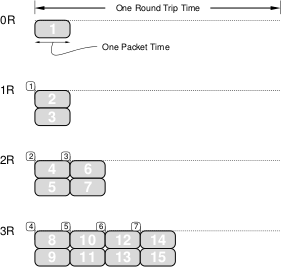
\includegraphics[width=0.48\textwidth]{img/slowstart}
  \end{center}
  \caption{The Chronology of a Slow-Start.\cite{JacobsonCAC}}
  \label{fig:slowstart}
\end{wrapfigure}

The idea behind bandwidth occupancy in TCP is to use as much as it is allow to
use. With this in mind, slow start proves the network by increasing
exponentially the rate of how many packets sends; the congestion window is
increases by one packet and adds another for each packet acknowledged. This
behavior continues until the slow start threshold (ssthrsh) is reached or
congestion is signaled. If congestion is detected, the slow start threshold is
reset to half of the amount of congestions window, at the time that congestion
window is reset to a size of one segment, and slow start is restarted. In case
that the slow start threshold is reached, the sender switches to congestion
avoidance mode, which is employed to maintain the transmission rate,
increasing by one segment each RTT\footnote{Each ack increases the congestion
window by $ss*ss/cwnd$. This results in a linear increase of the congestion
window; that means in 1 RTT, congestion window will be increased by
1 \cite{JacobsonCAC} \cite{rfc879} \cite{rfc2460}}.\\

TCP must be smart enough to signal to the hosts when path is experiencing
congestion, so it must have policies that decrease the network utilization or
increase it if congestion signals are received or not. Also, based on the
afore mentioned principle (``\textit{packet conservation principle}''),
congestion collapse would become the exception rather than a rule. Thus
congestion control involves finding place that violate conservation and fixing
them. It is important detect early this misbehavior, since new packets are
added exponentially also the congestion grows exponentially, so if is detected
early, only small adjustments will cure it.\\

Typically, when the sender is signaled that packets are been dropped, TCP/IP
networks understand that as congestion, but typical effects include queuing
delay, packet loss or the blocking of new connections. New implementations
define a explicit congestion notification methods \cite{rfc3168}, that allows
notification of congestion between the ends without any packet loss. TCP
specification mandates initially setting the congestion window to between 2
and 4 segments of data depending on the segment size\cite{rfc3390}.

\subsubsection{Congestion control algorithms}
One of the biggest problems that TCP had in the past years for its development
has been the achieve of optimal utilization preventing congestion associated
with the differences of bandwidth existing in the medium through which
communication is propagated. That is why lately there have been various
implementations for proper handling of the original algorithm originally
deployed in TCP for attaining prevent or lessen the effects of this problem.
Among the algorithms that currently exist, the two predominant in modern
operating systems will be mentioned: CUBIC and Compound TCP.\\

\paragraph{CUBIC TCP}  is the default implementation for congestion control in
the Linux kernel since 2.6.19. \textit{Scaling the window growth rate to match
large BDP\footnote{View definition in appendix \ref{app:definitions}} is rather
straightforward, tackling the fairness issues of new protocols has remained as
a major challenge.  Although BDP implies the network capacity by packet
count(or window size), packet count is not adequate to characterize TCP
performance because growth rate of TCP depends on RTT}\cite{HaCubic}.\\

Because the basis of their growth is a cubic function (hence its name), has a
less aggressive behavior than their predecessors, while retaining excellent
scalability, fairness and stability. As can be seen in figure
\ref{fig:cubicfunc}, the cubic function is compound of three parts: a concave
part where the window grows rapidly over small time values, a plateau set at the previous maximal
congestion window 

\begin{wrapfigure}{r}{0.5\textwidth}
    %\rule{5.5cm}{7.1cm}
\begin{center}
    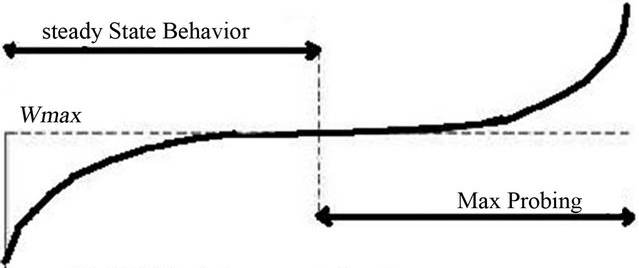
\includegraphics[width=0.48\textwidth]{img/cubic}
  \end{center}
\caption{The window growth function of CUBIC}
\label{fig:cubicfunc}
\end{wrapfigure}

\noindent size, and the end portion where the increasing bandwidth
above the maximum which exhibits a convex shape.\\

\begin{figure}[h]
\begin{minipage}{6cm}
\centering
	\[ W_{cubic} = C(t - K)^3 + W_{max}\]
    \caption{CUBIC's Congestion Window.\protect\footnotemark}
    \label{fig:cubicform}
\end{minipage}%
\end{figure}%

\footnotetext{C is a scaling factor, textit{t} is the elapsed time from the
last window reduction. $W_{max}$ is the window size before the last window
reduction. $K=sqrt[3]{W_{max}beta/C}$. And $beta$ is a constant
multiplication decrease factor applied for window reduction at the time of
loss event}

As can be better seen in the formula \ref{fig:cubicform}, the congestion
window ain't dependent of its previous acknowledged packets; instead, the
congestion window is computed at each step from a calibrated function. With
this calibration, the plateau is at the previous maximal congestion window
size. This feature allow the algorithm to respond faster to changes in
available bandwidth. Since in previous algorithms throughput is defined by the
packet loss rate as well as RTT, the throughput in CUBIC is defined by only
the packet loss rate.\\

Another feature that CUBIC has with respect to its predecessor in the Linux
kernel, it also changes the behavior of the Slow Start algorithm, replacing it
with one called Hybrid Slow Start (or HyStart)\cite{HaElephants}. The idea
behind this algorithm is to prevent the extra drop of packets caused by the
overshoot of bandwidth done by the regular slow start. This extra amount of
data cause unnecessary on both ends hosts and network, and taking long time to
recover from, that can be worst if the packet drop is made at a late stage of
the slow start\footnote{since slow start adds one extra packet for each
acknowledged}.\\

\paragraph{Compound TCP} under dev \cite{Tan06compoundtcp} and \cite{4146841}\\

\subsubsection{Fast retransmit and fast recovery} Timers are an important part
of this self-regulated protocol. TCP maintains four timers\footnote{The timers
that TCP has for each connection are: (1)Persist Timer: Ensures that window size information is transmitted even 
if no data is transmitted. (2)Keepalive Timer: Detects crashes on the other end of the
connection. (3)2MSL Timer: Measures the time that a connection has been in
the TIME\_WAIT state. (4)Retransmission Timer: The timer is started during a
transmission. A timeout causes a retransmission}.
One of them, the retransmission timer, causes the sender to retransmit the
segment over which at the expiry of this timer(which is a function of the
estimated RTT), has not yet received their respective acknowledge, assuming
the segment is lost in the network. When this action is unleashed, the server
will interpret it as a sign of congestion, but data still flowing.\\

As already seen in \textbf{2.2.2.1}, slow start can do a lot of damage to our networks, but fast retransmit helps to recover from lost without hurting the network that much. It is triggered after a specified number of acknowledgments, usually is at the third, with the same acknowledge number are received by the sender. This gives makes the sender reasonably confident that the next higher sequence number was dropped and needs to be retransmitted; all this without the need for the action triggered by the timeout.\\

Fast recovery manages the continuous transmitting of new data on subsequent duplicate acknowledgments, until the retransmitted packet is received. and after a non-duplicated acknowledge is received, the congestion window is reset back to the value it had before the fast retransmit was initiated, and the fast recovery mode is ended, going back to congestion avoidance mode.\\

%end TCP

\newpage

%section Buffers 
\section{Router's Buffers effects}
buffers

\subsection{Full Buffers}
%	1.- Full buffers: Couse no signals buffers at the right time, the buffers are always full
Packet networks require absorb bursty arrivals that TCP performs in order to
communicate two hosts. When received, a packet is immediately validated, but
not necessarily immediately processed and transferred out without kept in a
buffer. That means that if the rate at which packets are received is greater
than delay that takes to process and remove a package from the buffer, it
tends to fill up\footnote{When this occurs, the receiving device may need to
adjust window size to prevent the buffer from being overloaded.} and stay
congested, contributing to excessive traffic delay and losing the ability to
perfom their intended function of absorbing bursts.

This standing queue is the essence of Bufferbloat and is the result of the
difference between the window and the bandwidth of the link, only creating
long delays in communication, but no benefit in overall throughput. \textit{It
is not a phenomenon threated by queue or traffic theory, which, unfortunately,
results in it being almost universally misclassified as congestion(a
completely different and much rared pathology)}\cite{CACMStaff}.

When the packet reach a bottleneck queue, is squeezed down in bandwidth but
must strech out in time since its size stays constant.

\subsection{High Latency}
% 2.- Latency: When a new package arrives, it has to wait to the full queue get processed before its time, this way the package spent extra time waiting in the queue.
The latency a packet experiences in a network is made up of transmission
delay (the time it takes to send it across communications links), processing
delay (the time each network element spends handling the packet) and queuing
delay (the time spent waiting to be processed or retransmitted). But large
buffers only increase latency, and this only causes conflict with the needs
of nowadays applications.

Once packets in-fly reach a bottleneck, they begin to pool. Because the
characteristics already explained, more and more packets are coming, and this
queue continues to increase, which leads that each new arriving packet spending
more time in the queue than the predecessor packet, which means an
increase in the latency. Eventually, packets start to be dropped,
notifying the hosts of the presence of congestion on the path.

As stated in \cite{Dischinger2007CRB}, it is quite common to find these high-
latency queues in the last mile. The causes can be many, but among the most
common are both link quality at homes, as different implementations of traffic
shaping methods implemented by ISPs, or massive buffers set by the latter to
avoid loss of data, which can add a delay of up to several milliseconds.
Bottlenecks at the Internet's edge can easily move between the wireless
access (when its bandwidth is slow) and the provider's up-link, both of which
can have highly variable bandwidths.

For networks that use coaxial cable, multiple clients concatenated their
upward flows in a single transmission, resulting in a burst with a large
volume of data, which can led to a high fluctuation in latency. This
concatenation can also generate jitter time, which can be produce a miss
interpretation for some protocols of incipient congestion and cause to enter
into congestion control avoidance too early. The other type of highly used
networks are the DSL, which the more distance is between the supplier reduces
its transmission rate. That is why it is needed advanced signal processing and
error correction algorithms which can lead to high packet propagation delays.

\subsection{Sizing Router's Buffers}
Unmanaged buffers are more critical today since buffers sizes are larger,
delay-sensitive applications are more prevalent, and large downloads common.
Overly large, unmanaged, and uncoordinated buffers create excessive delays
that frustrate and baffle end users.

Correct buffer sizing is not an easy problem. Undersizing -- making buffers
smaller than the traditional BDP -- is fraught with problems. Today's links vary
in bandwidth, and individual connections vary in RTT. This makes it impossible
to properly pick a static size for most edge links. A simple, robust algorithm
that can manage buffer delay regardless of buffer size and link bandwidth
without a negative impact on utilization can make over-sized buffers
irrelevant.

A widely used rule-of-thumb recommends the buffers of size $B = \overline{RTT}
\times C $, where $\overline{RTT}$ is the average round trip time experienced by
connections utilizing the link, and $C$ is the data rate of the link. Many
buffers have been inserted without sufficient care due to the complexity of
establishing the appropriate size and test on real environments\cite{Vu-Brugier},
helping to determine where further complicate occurs Bufferbloat.

The rule-of-thumb comes from the idea of maintaining the medium as
busy as possible, and to maximize the throughput of the medium. But due to the
characteristics of TCP, no matter how large the buffer is, it will always be
saturated.

The main condition to choose the proper size of a buffer is the ability to
keep sending data in the periods in which the sender is stopped, preventing
possible downtimes in order to maximize utilization of the link and kept high
throughput at all times. The buffer will avoid to idle if the first packet
from the sender shows up at the buffer just as it hits empty.

After a lost is detected, the $cwnd$ is set to half of is last value, so if we
denote as $(W_{max} /2)/C$ the amount of time that packets are sent in
congestion phase, and as $B/C$ the time that takes a buffer with size $B$ to
drain, the size of a buffer $B$ needed is $B \leq (W_{max} /2)$
\cite{main:ref:1}.

The problem occurs when the required size buffers are implemented, and the
size is exceeded producing overbuffering. Overbuffering hurts anytime a link
is saturated causing extra delay, and destroying many uses of modern Internet.
As stated in \cite{GettysNichols}, \textit{a TCP connection must react quickly
to changes in demand at the bottleneck link, but TCP reaction time is
quadratic to the amount of overbuffering}.

Unfortunately this error comes from the fact that manufacturers began to think
that adding more buffer to their products should bring positive consequences,
especially considering the current volumes of data, in addition to providing
more equitable access to available bandwidth handled.

%end Buffers

\newpage

%section AQM
\section{Active Queue Management}
Ensure communication only checking the endpoints has revealed that it is not
enough and that it is also necessary to check the status of in-flight data
transmission. With the passage of time and with increasingly high speed
networks it has become more and more important to have mechanisms that keep
throughput high but average queue size low. The changes implemented in TCP for
congestion control have proven not to maximize the capacity of the medium
along with a performance degradation. Among the most common problems are:
connections still experience multiple packet loss, low link utilization and
congestion collapse. It is important to keep in mind that when a packet is
dropped before it reaches its destination, all of the resources it has
consumed in transit are wasted.

This is how the role of routers extends beyond joining and interconnecting local
networks and the Internet together. The role of routers becomes important
because they are able to better manage congestion that may occur in networks
due the knowledge they have about other routers in the network and can choose
the most efficient path for the data to follow, or as already seen, send
message to the ends to fall back or even drop data.  They must allocate
the available bandwidth fairly between all flows.

Typically the queues that routers maintain are designed to smooth and
accommodate bursts of data delivered by the hosts and transient congestion,
but as the queues start to fill, the routers drop packets using a FIFO based
drop-tail management. This discipline has two mayor drawbacks:
\begin{enumerate}
\item Lock Out: a small number of flows tends to monopolize the usage of the
buffer capacity\cite{evolvshortlongflows} .
\item Full Queue: these buffers tends to be always full, leading to 
high latency.
\end{enumerate}

Also, as explained in \cite{FloydJacobsonRED}, when a router use tail-drop,
\emph{the more bursty the traffic from a particular connection, the more
likely it is that the gateway queue will overflow when packets from that
connection arrive at the gateway/router}.

All this led to develop and implement more aggressive or active strategies for
congestion control on the Internet called Active Queue Management or AQM for
their acronym. AQM is a group of FIFO based queue management mechanisms to
support end-to-end congestion control in the Internet. The goals behind AQM
are to reduce the average queue length and with that decreasing the end-to-end
delay. Also to reduce packet losses that reflect as a more efficient resource
allocation.

AQM maintains the network in a region of low delay and high throughput by
dropping packets before queues become full and can reliably distinguish
between propagation delay and persistent queuing delay. Also, because the
router can monitor the size of the queue over time, the gateway is the
appropriate agent to detect incipient congestion. The most common AQM
algorithms are: RED, SRED, BLUE, SFB, CoDel.

\subsection{RED}
Random Early Detection or RED is the algorithm introduced in
\cite{FloydJacobsonRED}. RED monitors the average queue size and when it
exceeds a preset threshold, the router drops the arriving packet with a
certain probability, where the exact probability is a function of the average
queue size. If \gls{ECN} is active, the packets are choosen randomly and marked. When
a connection uses a larger share of available bandwidth, it is more likely to
be marked. The idle periods (periods when the queue is empty) are also take
into account for the calculations of the average queue size.

The objectives behind the  implementation of RED are:
\begin{enumerate}
\item Minimize packet loss and queue delay.
\item Avoid global synchronization of sources by randomize its marking
decision and by spacing out its marking.
\item Maintain high link utilization.
\item remove biases against bursty sources by limiting the queue occupancy so
that there is always room left in the queue to buffer transient.
\end{enumerate}

\begin{wrapfigure}{r}{0.5\textwidth}
  \begin{center}
    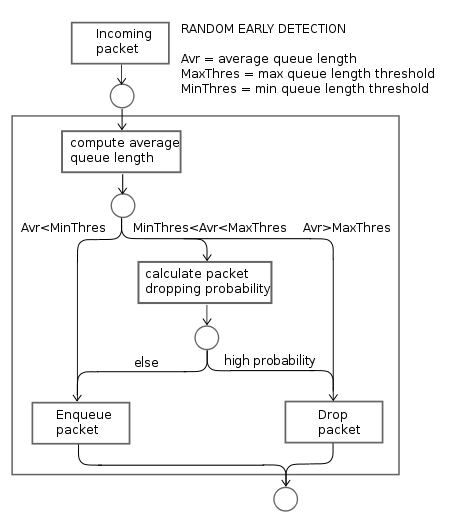
\includegraphics[width=0.48\textwidth]{img/RED}
  \end{center}
  \caption{RED's Flowchart}
  \label{fig:RED}
\end{wrapfigure}

Because RED can control the average queue size while accommodating transient
congestion, implementing RED in routers can provide high throughput and low
average delay in high-speed networks with TCP connections that have large
windows. Also, in routers where RED and ECN are implemented the bursty traffic
is well handled and the global synchronization between flows is avoided by
decreasing their window at the same time.

The most common critic to RED is its complexity to properly configure its
parameters. It is because of this that after their official publication, it
was necessary to perform a second publication \cite{NotesRED}, which aims to
explain a few more details on how to configure it properly. Since RED rely on
queue length as index of congestion, it can reflect the presence of congestion
but not the severity nor the numbers of competing connections sharing the
link. Since long ago networks ceased have a static configuration, RED require
a wide range of parameters to operate correctly under different congestion
scenarios. Unfortunately, this failure leads to deterministically mark packets
and suffer from poor link utilization. \textit{While  ECN timeouts allows RED
to avoid packet loss, the deterministic marking eventually causes
underutilization at the bottleneck link}\cite{FengBLUEAQM}.

As stated in \cite{NicholsJacobsonCQD}, \textit{RED was simple and can be
effective at reducing persistent queues, little guidance was available to set
its configuration parameters and it functioned poorly in a number of cases.
This led to a general reluctance to use it}.

Also to archive the ideal operating point, it can only do so when it has a
sufficient amount of buffer space, which leads to default induce an extra
latency.

\subsection{BLUE}
\begin{wrapfigure}{r}{0.5\textwidth}
    %\rule{5.5cm}{7.1cm}
    \centering
	\begin{verbatim}
	Upon packet loss
	    if (now - last_update >freeze_t)
	        Pm = pm + d1
	        last_update = now
	Upon link idle
	    if (now - last_update >freeze_t)$
	        Pm = pm - d2
	        last_update = now
  	\end{verbatim}
    \caption{BLUE's algorithm}
    \label{fig:BLUEAlg}
\end{wrapfigure}

Introduced by Wu-chang Feng et al in \cite{FengBLUEAQM}, BLUE aims to manage
congestion by using packet loss and link utilization history. The concept
behind BLUE's development is to avoid drawbacks of RED like parameter tuning
problems or to determine the fluctuations of actual queue length. The key idea
is to perform queue management based directly on packet loss and link
utilization rather than on the instantaneous or average queue lengths.

Through the use of a single probabilistic indicator called $p_m$, it
simplifies the process of dropping or marking packets when they are enqueued.
Against a continuous dropping of packets due to overflow, the probability
increases, increasing the rate at which it sends back congestion notification.
Also, to control how this parameter changes over time, the
$freeze\_time$ is used to determine the minimum time interval between
updates.  The value on which to increase or decrease, if the link is idle, is
determined by $\delta_1$ and $\delta_2$.

The effects of BLUE, as proved in \cite{FengBLUEAQM}, are the reduction of the
buffer size, which also reduces the end-to-end delay and helps to improve the
effectiveness of the congestion control algorithm. BLUE has also shown that it
has a better performance when marking incoming packets, leading to congestion
notifications causes periods of sustained packet loss nor periods of continual
underutilization.

\subsection{CoDel}
After several years using algorithms based on the average queue size, Nichols
and Van Jacobson realized that this approach although they have information of
congestion, no hard data on how serious is this. Jacobson et al, determined
that it may submit two types of queues: one that smooths bursts of arriving
packets turning it into a stable and continuous sent and tends to last less
than one RTT (called good queues); and those that only tend to create
excessive delays and lasting several RTTs (bad call queues). With this, they
were able to determine that the core of bufferbloat detection problem is
separating good from bad queues. Bearing in mind the above is that an
algorithm called \textit{Control delay} or CoDel by its acronym were
developed.

Presented in \cite{NicholsJacobsonCQD}, CoDel is based on the idea that it is
sufficient to maintain a threshold above which the tail can not exceed rather
than keeping a window of values to compute the minimum. Rather than measuring
queue size in bytes or packets, it is used the packet-sojourn time through the
queue. The time each packet spends in the queue is independent of the
transmission rate, the \gls{sojourn} is more valuable information about the behavior
of the buffer, in addition to being much more related to the effects you may
experience. The sojourn is based on a timestamp corresponding to when the
packet arrive to the queue, at which this mark is added to the package
information. The minimum packet sojourn can be decreased only when a packet is
dequeued.

Another difference that occurs is that CoDel accepts the existence of queues,
but it is unacceptable to drop packets when you have a buffer with less than
\gls{MTU}'s bytes.

\begin{wrapfigure}{r}{0.5\textwidth}
    \centering
	$f(n) = \frac{100}{\sqrt{n}}*f(n-1)$ \\
	f(0) = 1
    \caption[CoDel droptime interval]{CoDel droptime interval, n=iteration}
    \label{fig:CoDeldroptime}
\end{wrapfigure}

But when the queue delay has exceeded target for at least interval, a packet
is dropped and a control law sets the next drop time accordingly to Figure
\ref{fig:CoDeldroptime}. The ways in which CoDel stops packet drop is either
when the delay queue is less than the target value or when the buffer contains
less than MTU's bytes. Furthermore the algorithm has additional logic that
controls reenter to dropping state too soon.


Beside the minimum packet sojourn, the other two parameters that CoDel needs
are the target and interval, which are almost self-explanatory. Target is the
acceptable standing queue delay and interval works as the  time on the order
of a worst-case RTT of connections through the bottleneck. The recommended
target value is 5ms since tests reveal that with this value, the utilization
of the links is the optimal. Interval is loosely related to RTT since it is
chosen to give endpoints time to react without being so long that response
time suffers. A setting of 100ms works well. \textit{CoDel's efficient
implementation and lack of configuration are unique features that make it
suitable for managing modern packet buffers}\cite{NicholsJacobsonCQD}.

%end AQM

\newpage

%Flaws
\section{Hidden Flaws and Bufferbloat}
Because much of the basis for how TCP was designed in the early days of the
Internet, where speeds were low, the burden on the networks were only a few
kbps, and the networks interconnecting were separated by a couple
milliseconds, the use was ideal. But it is not hard to see that in the past
few decades, Internet growth has exceeded the expectations of even the most
experienced analysts and dreamers.

Intensive-consumption applications like on-line games, audio and video
streaming for music or on-line calls, torrent or P2P applications and 
sites that have a high level of resource utilization like Youtube, Facebook or
Netflix, have made networks of today quite different from those that formerly
existed, but still running the same protocols\footnote{While many have been
updated, the basics remain the same}. If that was not enough, the creation and
incorporation of new devices such as smart phones, tablets and even smart-watches
with the ability to transmit data over the Internet, makes more necessary a 
wealth handling of information in an efficient and properly way.

TCP relies on timely notification to adjust its transmission rate to the
available bandwidth, which is commonly signaled by the packet loss. But since
couple of years, and helped by lower prices on hardware manufacturing along
with the thought that more is always better, the manufacturers had decide to
prevent as much as possible the loss with the addition of larger buffers on
their devices. This simple action is slowly bringing a new collapse not only
TCP but data transmission in general, as can be seen in \cite{CACMStaff}

With the increase in the size of buffers, the packages spent more time
``on the fly'' in this big buffers instead of dropped, signaling to TCP to
reduce the sending rate. When this large amount of data is dropped, causes TCP
sharply drop in transmission rate, freeing up bandwidth. Unfortunately, due to
the size of the buffers is static, when the new TCP slow-start phase start,
again due to the lack of signals out of time, TCP will work with diminish
performance. This problem is cyclical, resulting in exponential TCP back-off,
throughput degradation and very high latency

But the paths on Internet are shared by multiple TCP streams so the buffers,
and this back-off behavior has a tendency to synchronize flows
\cite{main:ref:1}. This cause all the flows to throttle back their
transmission rates simultaneously, amplifying the effect. This decrease in
latency and reduced throughput are the effects of Bufferbloat phenomenon.

As stated in \cite{GettysNichols}, \textit{long delay from Bufferbloat are
frequently misattributed to insufficient bandwidth and this misinterpretation
of the problem leads to the wrong solutions being proposed}. As seen in the
past sections, the packet loss for TCP is not in itself a problem, conversely
it is essential for its functioning. The real problem is  the excessive and
consecutive packet losses that occurs when the buffers kept persistently
fulls. This effects may cause that modern applications timeout their
connections or in others may experience some delay. This is the real
effects and problems of Bufferbloat.

%end Flaws

\newpage

%section Test
\section{Experimental Work}
The goal of the experiments outlined in this section is to examine different
residential and public networks with the objective to proof the existence of the
phenomenon under an uncontrolled scenario. This will be done by running a set of
tests with different tools, first to define and characterize the network, then
to measure and compare how the network behave with and without load. More
specifically, the factor to be tested is the latency under load and analyzed to
identify if the latency that occurs is due to an excess of buffers or due to
some other problem.

This section aims to explain the setup that will be used to perform the tests,
the selected tools for each of these tests and what is to be achieved and 
expected from each one of these tests.


\subsection{The Test Setup}
The tests were ran under a pseudo controlled environment, using one
physical  machine and a second virtual machine hosted on the first machine. These
systems runs under a regular OS without any modifications. Also, for some tests two other devices will be
added,  one acting as an Iperf Server and a regular Android Tablet that will
be used to add some extra load to the network when the Ethernet cable is used
as medium.

All of these tests will be carried out in a real-world scenario, where no
packet  prioritization is done by the server against our flows, the routes can
vary between each iteration of the same test, and many different flows will
collide with other flows from different sizes and types. Nor there is more
information about how the flows are treated by the queue manager algorithms or
about how they are  configured.

\subsubsection{Hardware Characterization}

\begin{description}

\item [Physical Machine]: \hfill \\
The physical machine runs as host OS, Windows 7 SP1, that works with an Intel(R)
Core(TM) i7-2670QM CPU \@ 2.20GHz with 8GB of available RAM. This machine will 
always be connected through its wireless adapter, a \textit{Broadcom Corp. 
BCM4313 802.11b/g/n Wireless LAN Controller (rev 01)}. The Ethernet controller 
is a \textit{Realtek Semiconductor Co., Ltd. RTL8111/8168 PCI Express Gigabit 
Ethernet controller (rev 06)} adapter, and will be bridged to the virtual 
machine for some tests.

\item[Virtual Machine]: \hfill \\
The virtual machine is hosted using VMWare Player 6.0.1, with 4 processors 
assigned for use plus 4GB of RAM, and with the Ethernet adapter connected only
for certain tests. The OS selected is a Debian based OS called Kali Linux, and
using the kernel release identified as Debian 3.12.6-2kali.

The wireless adapter is a AIR-802 USB adapter with Zydas chipset and a TP-link
8dbi antenna. This adapter is directly connected to the virtual machine and
hooked to the physical machine without the USB extension, this way any extra
signal  loss is avoided. 

\item[Iperf Server]: \hfill \\ 
This is a VPS hosted by Digital Ocean
\footnote{\url{https://digitalocean.com}} with 512MB Ram, 20GB SSD Disk, and
located in New York data center. This machine runs Ubuntu 12.04.3 x64 under
KVM software using as a processor an Intel Hex-Core 3 GHz.

\end{description}

The idea of using an external device to connect the virtual machine to the 
network and not using a bridged configuration provided by software, is mainly 
because with an USB device the machine will take care of all the management and 
administration of the device, avoiding any possibility that the host machine 
modifies or manages any flow. Also, by using a second machine to overload the 
uplink avoids overflow the queue on the machine that is performing 
the tests. With this, it is expected to minimize the possibility that our 
testing machine is causing extra latency, either by the saturation of the 
wireless channel, or by the queue in the traffic control subsystem into the 
kernel. 

For the tests, the Bufferbloat community\cite{bloat} has created a set of best 
practices\cite{tg12} to follow so the results are consistent and repeatable, 
but in this case, computers and routers will not be modified as it will attempt 
to analyze what an every-day-user experience. Those practices will be taken in 
consideration if it is the QOS present in routers and deactivate as recommended.
 


\subsection{Tools Definition}
The tools used for the benchmark were selected by the capability to
determine  the presence of the Bufferbloat phenomenon in the network of
study. So, with this as a main consideration, the
tools selected for  the benchmark will be chosen by the complexity and
accuracy to measure and  determine the RTT into an IP/TCP connection, and how
hard is to consistently  replicate the results under similar contexts. Other
tools were selected to help  determine, characterize, and prove the capability
of the network to cause  Bufferbloat.

\newpage 

The tools selected to be used in this tests are the following:

\begin{itemize}
    \item Speedtest test by Ookla
    \item Netalyzr by ICSI
    \item Iperf Tool with Tcptrace/Xplot.org
    \item Page Benchmarker extension for Google Chrome
    \item Smokeping Latency Tool
\end{itemize}

\subsubsection{Speedtest}

Developed by Ookla\footnote{\url{https://www.ookla.com/about}}, this tool is used
for most of the ISPs and many users in Chile to test their broadband's
connections globally. It can be used not only in their website 
\href{http://www.speedtest.net}{\emph{www.speedtest.net}} but also on Android,
iOS or Windows Phone. A command line interface developed in Python can be used 
too for testing Internet bandwidth.

The server selected to perform every test, either has or not the
fastest ping, is the one hosted by the Pontificia Universidad Cat\'olica de
Valpara\'iso (this host is the default selected most of times by the site also).  

\subsubsection{Netalyzer}

For end-users, little is revealed about how ISPs manage their networks. That is
why since 2009 ICSI has developed Netalyzr, a ``two click '' tool developed to
test networks that runs in web browser as a Java applet. Once downloaded, the
applet contacts the back-end server using a range of protocols and mechanisms
employed as part of the testing, and then conducts a series of tests. Once
completed, it uploads its findings to the back-end where they are distilled
into a detailed report breaking down the findings into correctly operating
aspects, those that show potential signs of trouble, and those that are
downright broken. Figure \ref{netalyzr_ex} is an example of the output.

\begin{wrapfigure}{r}{0.5\textwidth}
	\begin{center}
		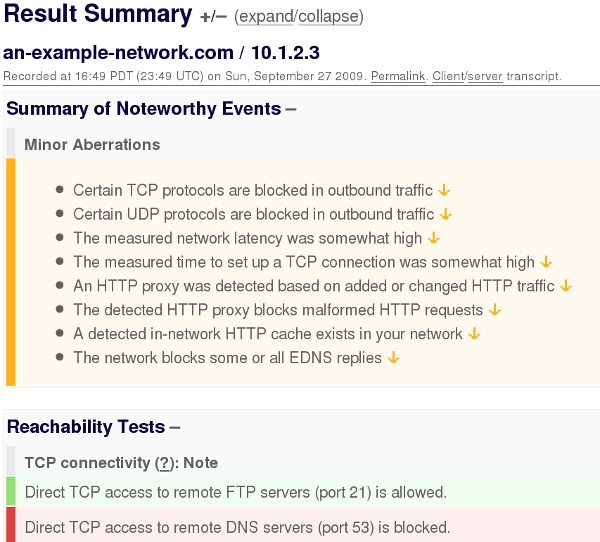
\includegraphics[width=0.48\textwidth]{img/netalyzr_ex}
	\end{center}
	\caption[Result Summary example from Netalyzr]{Result Summary example from Netalyzr. Source:
	\url{www.dslreports.com}}   
	\label{netalyzr_ex} 
\end{wrapfigure}

The primary goal in developing Netalyzr's tests was to provide a new kind of
diagnostic tool, \emph{one that particularly illuminates under what sort of
restrictions a user's Internet connection operates, like both forms of filtering
(blocking) and proxying imposed by the user's ISP, and performance issues that
arise from the nature of the user's Internet access setup}\cite{netalyzr}. Among
the performance considerations, Netalyzr's measures are packet loss, latency,
bandwidth. Also, it compute in-path forwarding device buffer size by comparing
small-packet latencies under idle and loaded states in networks (the perfect
time to occur Bufferbloat). Other tests like general TCP and UDP service
reachability are performed.

\subsubsection{Iperf}
Iperf is a well known and commonly used network testing tool. It can create a
TCP and UDP data streams and measure the bandwidth and the quality of a network
link. It can perform multiple tests like Latency, Jitter or Datagram Loss.

Iperf basically tries to send as much information down a connection as quickly
as possible reporting on the throughput achieved. This tool is especially useful
in determining the volume of data that links between two machines can supply.
This two machines define the network, one acting like a server and the second as
the client. For this scenario, the server will be the VPS that only will receive
the Iperf connections (also will be running ssh but without further
interaction). The VM Linux machine will work as an Iperf Client.

As mentioned in Iperf users mailing list ``\emph{When one runs TCP tests,
there are 2 things that block Iperf from having clear view of real throughput:
buffering on sender's side (TCP/IP stack) and TCP behavior itself (acking).
What Iperf can measure is the pace with which it sends data to TCP/IP stack;
TCP/IP stack will only accept data from application when buffers are not full.
If the buffer is huge, Iperf will see high throughput initially, then it will
drop. If there's congestion or retrasmission going on, Iperf will see it as
lower throughput}''\cite{iperfmaillist}, but the data generated by Iperf won't
be further analyzed because the  idea behind using this tool is a TCP's packet
generator. This means that the packets generated by  Iperf will captured and
analyzed with tcpdump, tcptrace and xplot.org.

\subsubsection{Page Benchmarker}
Page Benchmarker is a Google Chrome extension that intent to test page load 
time performance within Chrome. Measures time-to-first-paint, overall page load 
time, KB read/written, and several other metrics, and with its capability to 
clear the cache and existing connections between each page load, makes this 
tool one of the main sources of income to analysis.

\subsubsection{Smokeping}
SmokePing is a latency logging and graphing tool that consists of a running 
daemon which organizes the latency measurements and a CGI which presents the 
graphs. SmokePing give us the ability to measure latency and packet loss 
in the current network, and with RRDtool, is capable to maintain a long term 
data store and to draw different graphs with the giving up-to-the-minute 
information on the state of each network connection.

Smokeping can be configured to perform a wide range of latency measurement 
probes each one directed to an independent target or over a set of targets 
selected for each proof.


\subsection{Test Description}
description

	
%end section Test
\newpage
%section Results
\section{Results}
This section shows and summarizes the results obtained in the different tests detailing each specific case, and then collect and summarize all.


\subsection{Speed test}
As expected, in all cases the networks were asynchronous, being significantly
higher the bandwidth related to the download (the downlink) than the uploading
or uplink. This also explains the relationship between the uplink and ping,
presenting a major ping in the networks with lower uplink. The relationship
can be better be seen in the Figure \ref{fig:speeds}.

\begin{figure}[ht]
\centering
	%\rule{5.5cm}{7.1cm}
    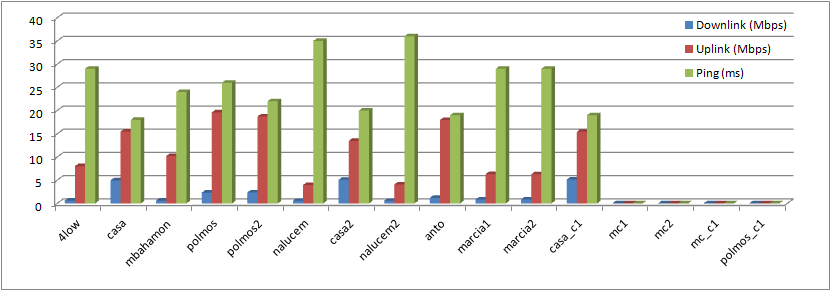
\includegraphics[width=0.9\textwidth]{img/speed_graph}
\caption{Speed and Pings based on Appendix \ref{app:bwmeasures}, Table \ref{table:speeds}}
\label{fig:speeds}
\end{figure}%

The Figure \ref{fig:speeds} also is a prove of the common missundersanding
about the how the ISP's promote high download speeds but with low uplink. Even
though most of the time home users download content, in order to keep a good
ratio the data needs to flow between both sides, because due the way TCP
works, you need good communication in both directions. While in theory this
works without major problems, unfortunately in reality users download content
from different sources at once, and if we add the new requirements like in
real-time  or on-demand applications and online games, we see that not only a
high downlink is important.

Another important point is the growing need for higher bandwidth capacity.
Unfortunately it is common to associate bandwidth with speed. Instead,
bandwidth is a measure of capacity, not how fast the network responds. Then,
more capacity is only better if the existing latency is lower. This may
explain why the tests performed in network tagged as \textit{``casa''} can have low pings
even when its capacity is close to the mean, but this network is through
fiber\footnote{In practice, fiber service have a propagation delay 10 times
faster than ASDL service}.

\begin{table}[ht]
\begin{center}
\begin{tabular}{|c||c|c||}
 \hline
& \multicolumn{2}{|c|}{Ratio (\%)} \\ \hline
Location	& Uplink		& Downlink \\ \hline \hline
casa\_w		& 99,00			& 103,20 \\ \hline
casa2\_w	& 101,80		&  89,73  \\ \hline
casa\_c		& 103,00		& 102,93  \\ \hline
marcia\_w	& 166,00		&  63,00  \\ \hline
marcia\_c	& 166,00		&  62,90  \\ \hline
sara\_w		& 112,00		&  54,50  \\ \hline
sara\_c		& 114,00		&  80,80 \\ \hline
polmos\_w	& 116,00		&  49,03  \\ \hline
polmos2\_w 	& 117,00		&  46,80  \\ \hline
nalucem\_w	& 114,00		&  99,25  \\ \hline
nalucem2\_w & 112,00		& 101,50  \\ \hline
mbahamon\_w & 120,00		& 102,10  \\ \hline
4low\_w	 	& 120,00		&  80,30  \\ \hline
hidalgo\_w 	& 119,00		&  89,80  \\ \hline
\end{tabular}
\caption[Speed Test: Variation ratio of offered vs measured speed ]{Variation ratio of offered vs measured speed.}
\label{table:ratiospeed}
\end{center}
\end{table}

The $\sim12ms$ ping were also not obtained, but the values ​​are still within
the acceptable range around the $\sim26ms$. These values ​​may be due to
factors such as congestion, conditions on the server, or the processing time
information. The variation of the ratio between the measured and the bandwidth
contracted is of 80\%, which is only 6\% less than the spected
value\footnote{Details of the provider and bandwidths can be found on Appendix
\ref{app:bwmeasures}, Table \ref{table:comparative}}.

Further analysis is needed to determinate how the bandwidth is related with
the Bufferbloat, but it is clear that less the bandwidth, higher the ping, but
it can not be stated the oppossite, higher the bandwidth, less the ping
becouse it also depends on how fast the network is and the effects in the
latency \cite{main:ref:3}.


\subsection{Netalyzr test}
After having a clear idea about the capacity of the network, it is necessary
to know how it speed and behavior works. This requires to analyzing how
latency behaves. As stated, latency is the time it takes a message to travel
from one computer to a sever, and has a huge impact on how the user experience
the network.

Within all the information that Netalyzr provides, it only will be taken only
the most relevant information to determining whether Bufferbloat is presented
on our networks. For this, the data that will be take into consideration is:

\begin{description}

\item [DNS resolver Time:] This test intent to measure how quickly the DNS
resolver is able to resolve the mnemonic name. Slow resolvers may make the
network seem ``slow'' even if the network itself is fast.

\item [Network Buffers:] The most revealing fact of the existence of the
phenomenon studied. While it is a fact that is commonly overlooked, also it is
crucial to the quality of the network. If the buffer is too small, network
protocols such as TCP are unable to send as fast as the network allows. If the
buffer is too large, a single transfer will fill up the buffer, delaying all
other traffic.

\item [Network Performance:] To determine the performance of the network,
Netalyzr measures latency by sending a series of small messages to the server
and then seeing how long it takes the messages to return. Since the
communication if from outside US, the latency should naturally be higher, but
how much higher?
\end{description}


The results in Table \ref{table:buffer} are much more clarifying than those
obtained in the previous test. In the first data set related with DNS, the
times are relatively stable and the time that took to resolve the requests
were almost indiscernible. While it is common to find cases with shorter at
$\sim15ms$ for local name resolution\footnote{ As example can be a site hosted
in the same country and tested with dig -
\url{http://linux.die.net/man/1/dig}}, the average resolution time is
acceptable within the metrics for international queries. A special case is
presented on the network tagged as \textit{``4Low''} were the time that take
to effectively resolving queries to any website is extremely high but after
the resolution finish, the network looks as had no major problem in data
acquisition. Also no mayor relation can be seen between the bandwidth and the
DNS resolve time.

\begin{table}[ht]
\begin{center}
\begin{tabular}{|c||c||c|c||c|c||}
 \hline
& & \multicolumn{2}{|c||}{Buffer} & \multicolumn{2}{|c||}{Performance} \\ \hline
Location	& DNS (ms) 	& Uplink (ms)	& Downlink (ms) & Latency (ms)	& Loss (\%) \\ \hline \hline
casa\_w		& 190		& 290			& 190 			& 140			& 00,00		\\ \hline
casa2\_w	& 180		& 280			& 180 			& 140			& 00,00		\\ \hline
casa\_c		& 180		& 280			& 190			& 140			& 00,00		\\ \hline
marcia\_w	& 190		& 1200			& 860			& 190			& 0,50 		\\ \hline
marcia\_c	& 180		& 990			& 2100			& 190			& 00,00		\\ \hline
sara\_w		& 220		& 5100			& 470			& 160			& 4,00 		\\ \hline
sara\_c		& 200		& 5100			& 459			& 160			& 4,00 		\\ \hline
polmos\_w	& 220		& 360			& 160			& 180			& 00,00		\\ \hline
polmos2\_w	& 180		& 370			& 160			& 190			& 00,00		\\ \hline
nalucem\_w	& 210		& 5100			& 1800			& 160			& 1,50 		\\ \hline
nalucem2\_w	& 210		& 5100			& 1800			& 210			& 0,20 		\\ \hline
mbahamon\_w	& 200		& 2900			& 290			& 200			& 1,50 		\\ \hline
4low\_w		& 1300		& 2900			& 590			& 180			& 0,50 		\\ \hline
hidalgo\_w	& 180		& 260			& 100			& 200			& 1,50 		\\ \hline
\end{tabular}
\caption[Netalyzr Test:DNS resolution time, Buffer time and Performance]{DNS resolution time, Buffer time and Performance}
\label{table:buffer}
\end{center}
\end{table}

The next four lines are crucial to proof existence of the phenomenon. The
buffer section can reveal how much time a packet spent in the existing buffers
along the way or, in other words into the link between the network and the
server. Unfortunately, in the uplink times are about $\sim300ms$, which
according by ICSI are times that in some cases may present a degraded
performance (as in online games or real time conference). For the downlink,
the networks that already are marked with high buffering time in the uplink
are the same for the opposite route. While the high measured times in the
uplink could it be justified by the diminish capacity to put new data in the
network against the capacity related with the downlink (related with the
asynchronous bandwidth capacity) there are cases in which the time is
excessive and Netalyzr alert the presence of excessive buffers possibly
generated by Bufferbloat.

\begin{table}[ht]
\begin{center}
\begin{tabular}{|c||c|c||}
 \hline
 & \multicolumn{2}{|c||}{Bandwidth (Mbps)} \\ \hline 
Location 	& Uplink & Downlink			   \\ \hline \hline
casa\_w		& 5,00	 & 14,00			   \\ \hline
casa2\_w	& 5,00	 & 14,00			   \\ \hline
casa\_c		& 5,00	 & 15,00			   \\ \hline
marcia\_w	& 0,47	 & 1,50			   	   \\ \hline
marcia\_c	& 0,54	 & 6,20			   	   \\ \hline
sara\_w		& 0,57	 & 6,30			   	   \\ \hline
sara\_c		& 0,57	 & 6,30			   	   \\ \hline
polmos\_w	& 2,10	 & 9,60			   	   \\ \hline
polmos2\_w	& 2,10	 & 9,60			   	   \\ \hline
nalucem\_w	& 0,57	 & 4,00			   	   \\ \hline
nalucem2\_w	& 0,57	 & 4,00			   	   \\ \hline
mbahamon\_w	& 0,54	 & 7,80			   	   \\ \hline
4low\_w		& 0,54	 & 6,60			   	   \\ \hline
hidalgo\_w	& 1,00	 & 11,00			   \\ \hline
\end{tabular}
\caption[Netalyzr Test: Bandwidth]{Bandwidths measured with Netalyzr}
\label{table:Bandwidth}
\end{center}
\end{table}


The main characteristic of Bufferbloat is the high latency, with some effect
on the packets loss, since packets spends most of the time in buffers along
the route. Netalyzr actually reveals that in at least two networks,
\textit{marcia} and \textit{sara}, this phenomenon occurs because although the
latency is low under normal conditions there is packet loss and buffer times
higher than normal. The packet loss can also be due to the conditions of the
experiments, and because due its characteristics, it is more common higher
packet lost using wireless but for these experiments there were no obstacles
between the router and computer located less than a meter from each other. Also
it is important to remember that the way of buffering time and latency are
calculated is through two different experiments with low and high load on the
network.

Among the characteristics of Netalyzr is the capacity to introduce a summary
table where it can be seen the different problems that arise in the networks
and the severity thereof. In Table \ref{table:Errores} are presented the
summary after all networks.

\begin{table}
    \begin{subtable}{\linewidth}
    \centering
    \caption*{Panel A: Summary or errors}
    \begin{tabular}{|c||c|}
 \hline
Location		& Alerts            \\ \hline \hline
casa\_w			& 1,2,8             \\ \hline
casa2\_w		& 1,2,8             \\ \hline
casa\_c			& 1,2,8 			\\ \hline
marcia\_w		& 1, 3, 6, 9 		\\ \hline
marcia\_c		& 1, 3, 6, 8, 9 	\\ \hline
sara\_w			& 1, 2, 4, 5, 6, 8 	\\ \hline
sara\_c			& 1, 2, 4, 6, 8 	\\ \hline
polmos\_w		& 1,8 				\\ \hline
polmos2\_w		& 1, 3, 6, 8 		\\ \hline
nalucem\_w		& 1, 2, 6, 8 		\\ \hline
nalucem2\_w		& 1, 2, 6, 8, 10 	\\ \hline
mbahamon\_w		& 1, 3, 6, 8, 10 	\\ \hline
4low\_w			& A, 1, 3, 6, 7, 8 	\\ \hline
hidalgo\_w		& 1, 8 				\\ \hline
    \end{tabular}
    \end{subtable}
\bigskip
    \begin{subtable}{\linewidth}
    \centering
    \caption*{Panel B: Description of errors}
    \begin{tabular}{|c||c|}
 \hline
 \multicolumn{2}{|c|}{Alerts} \\ \hline \hline
A	& ISP's DNS is slow to lookup names								\\ \hline
1	& Certain TCP protocols are bloqued in outbound traffic 		\\ \hline
2	& The network does not reply when it needs fragmented traffic 	\\ \hline
3	& Fragmented UDP traffic if bloqued 							\\ \hline
4	& The packet loss was somewhat high 							\\ \hline
5	& The time to set up a TCP connection was somewhat high 		\\ \hline
6	& Network packet buffering is excessive 						\\ \hline
7	& DNS resolver may have probelms with DNSSEC 					\\ \hline
8	& Only some root servers returned DNSSEC information 			\\ \hline
9	& Not all DNS types were correctly processed 					\\ \hline
10	& The network indicated bursts of packet loss 					\\ \hline
\end{tabular}
\end{subtable}
\caption[Netalyzr Test: Summary of errors and warnings in Netalyzr]{Summary of errors and warnings in Netalyzr}
\label{table:Errores}
\end{table}

With this summary is easy to clarify that the networks mentioned noted
actually have problems with the time with their buffers, specifically troubled
networks are: \textit{marcia, sara, nalucem, mbahamon} y \textit{4low}.
Coincidentally, less bandwidth networks are the same with longer buffers. In
addition, as mentioned, the network \textit{4low} also has serious issues
with the name resolution.



\subsection{Iperf test}
Since the networks are already characterized and with enough knowledge to
define which networks the phenomenon studied  is mostly likely to occur
theoretically, the following are the results of the first part of the
practical experimentation.

Iperf revealed that indeed, overloading a network average RTT time in direct
proportion to the load in-fly (relation with more data to negotiate, more
information over the network, higher RTTs), with which to demand it even more,
like including other connections can reach to the collapse making even to load
a basic website will become a task that takes a couple of minutes.

The following graphs show results in three networks characterized in ascending
seriousness of the problem. Each figure is the result of three iterations
performed in each network, without load and the two iterations performed with
extra load.

\begin{figure}[ht]
\centering
	%\rule{5.5cm}{7.1cm}
    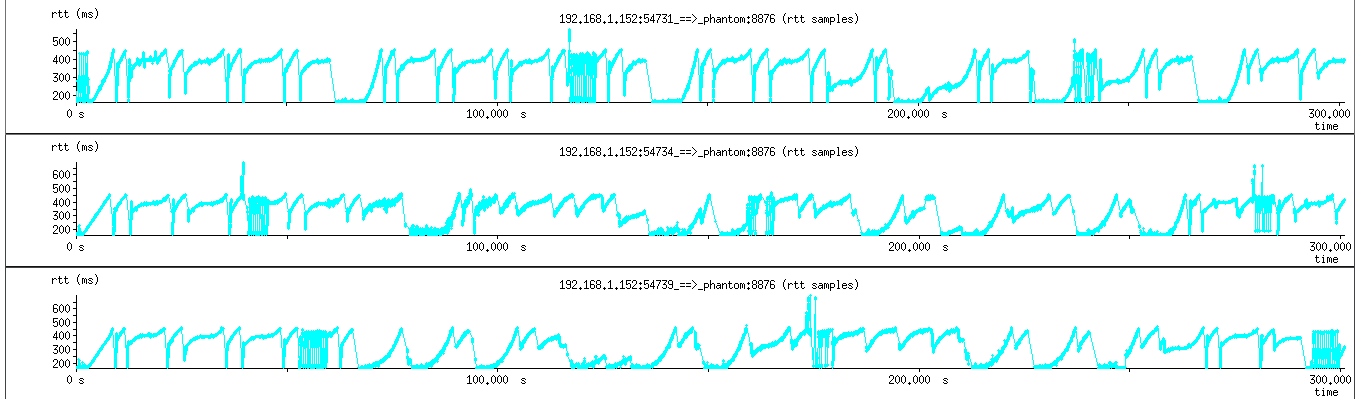
\includegraphics[width=\textwidth]{img/n_iperf_good}
\caption[Iperf: RTT graphs for a fiber network]{RTT graphs for the three test in a fiber network}
\label{fig:iperfgood}
\end{figure}%

Figure \ref{fig:iperfgood} shows the behavior of the network which, although it
has a bandwidth in the mid-high average range, but with its transmission rate
higher because it is a fiber optic network (\emph{casa\_w}). It can be
appreciated that in a state where only one application uses the entire
bandwidth, there is an increased RTT time, but not significant. In fact the
only difference compared to the following two graphs sharing network resources
applications is that there are some higher peaks, but these are not constant.
Nor is there a greater retransmission (denoted by the thinner lines). So, with
at least two data sources generating traffic, there is no significant increase
in RTT time and should not imply that the increase in the loading time for a
browsing client, or some type of problem seen in real time applications.

\begin{figure}[ht]
\centering
	%\rule{5.5cm}{7.1cm}
    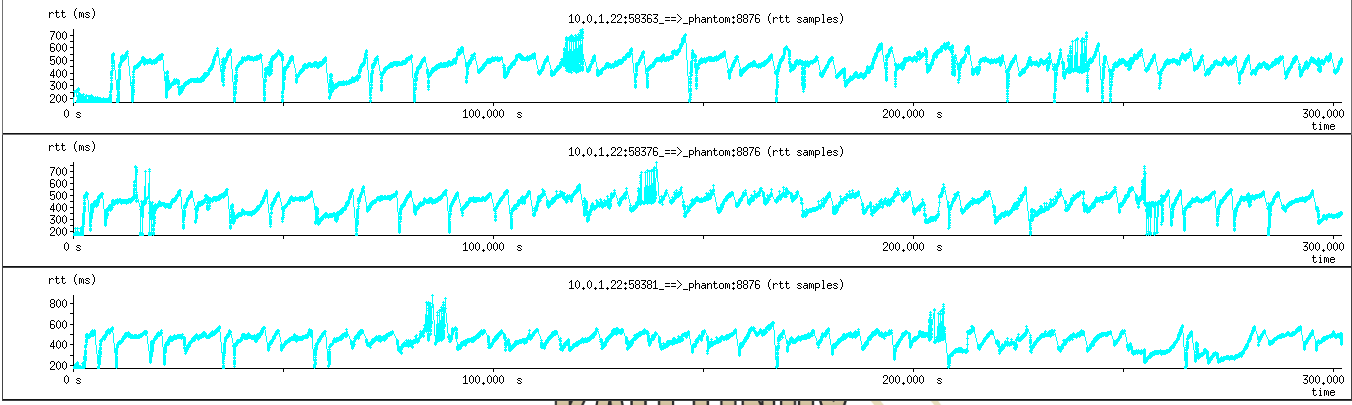
\includegraphics[width=\textwidth]{img/n_iperf_mid}
\caption[Iperf: RTT graphs for a network with minor issues]{RTT graphs for the three tests in a network with minor issues}
\label{fig:iperfmid}
\end{figure}%


For Figure \ref{fig:iperfmid}, at the beginning of the fist test (first $\sim10$ seconds) the RTT times are really small, but according to previous cases, is about the time it takes to saturate the buffers. This behavior proves that is what is occurring, specially that after this period of time RTT rise almost doubling, presenting ranges between 400 and 700 ms, but with valleys that are round to  300 ms or less. For the second and third graph in this network, the valleys are reduced and with higher values, especially in periods when the second application is making use of the resource (between about 50 and 250 seconds), being noticed particularly few times in the third chart which also shows an increase in the maximum upper 800 ms. This network corresponds to \emph{polmos\_w}.

\begin{figure}[ht]
\centering
	%\rule{5.5cm}{7.1cm}
    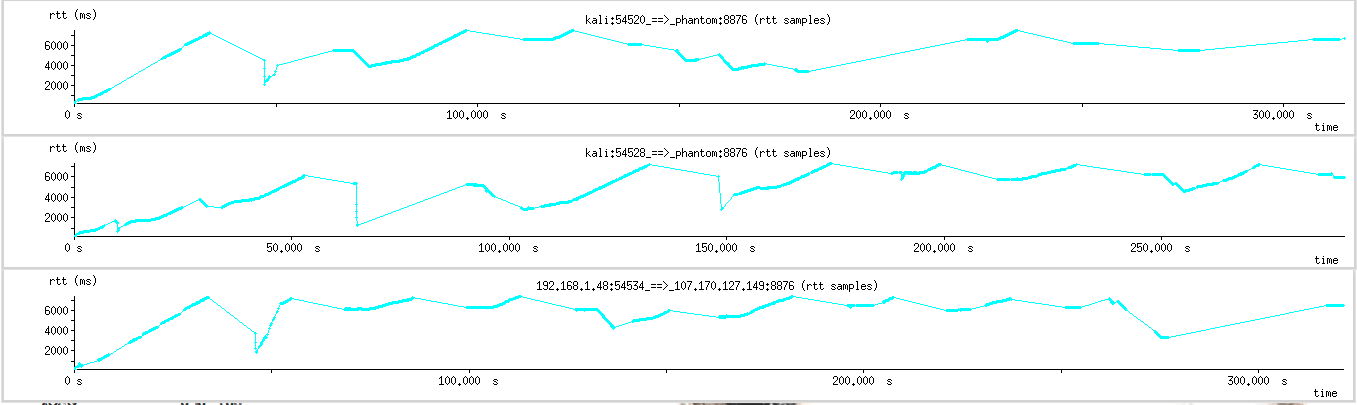
\includegraphics[width=\textwidth]{img/n_iperf_bad}
\caption[Iperf: RTT graphs for a network with bad performance]{RTT graphs for the three tests in a network with bad performance}
\label{fig:iperfbad}
\end{figure}%

In Figure \ref{fig:iperfbad} the things got to the extreme. Even for the base
case, where the times should be low, for this scenario the peaks are around 6
seconds, with a always upward trend. Also it is a constant presence of long
periods where no samples are among the packets in transit which are not
retransmitted packets (thinner lines). Current websites delayed an average of 2
seconds to load the full site, finding in the range between 1 and 7 seconds,
for the full negotiation; but in here, only one package is taken almost the
same that takes a full site to load.

At first glance it seems that the case two is better than the base case, but
it can be notice the relay times (may be caused by loss), are up most of time,
perhaps they produced a massive drop of packets (approximately the second 70),
so having a valley at a point less than in the base case. The third graph
shows no far difference with what already found only proving the fact that
there are some serious problems in the network that makes RTTs times increase
to three or four times the normal behavior. With this times, it is almost
impossible to maintain a steady stream of data with one application, so the
use of real-time applications such as online games or web conference while web
surfing would be almost impossible, and must sacrifice any.

\begin{figure}[ht]
\centering
	%\rule{5.5cm}{7.1cm}
    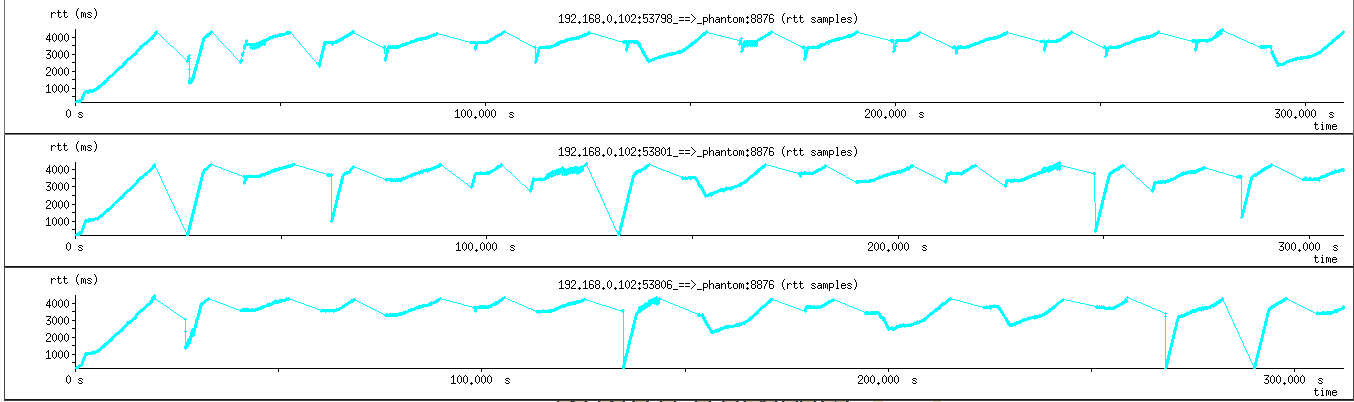
\includegraphics[width=\textwidth]{img/n_iperf_4low}
\caption[Iperf: RTT graphs for a network with DNS issues]{RTT graphs for the three tests in a network with DNS issues}
\label{fig:iperf4low}
\end{figure}%

It is interesting to mention that for the network \emph{4low}, which presents problems with DNS resolution time was needed more than twice tries in order to perform this tests, as the website used to saturate as a second stream of data could not be loaded throwing error connection time (timeout). After the website complete its full load, having to load it before start iperf for the two cases, it could continue with the normal course of the test.


\subsection{Benchmark test}
While ordinary Internet users request mainly optimized  web sites to make the
most of each user connection, it is natural that the traffic generated by
several requests of web sites simultaneously generates some kind of significant
load to the network. Or so it is what one should naturally think.

Unfortunately with the results obtained with this Page Benchmark it is more
clear to see it is not so. By analyzing Figure \ref{fig:loadmeans}, the
networks that already were categorized as \textit{with problems}, follow that
trend and even with all the available bandwidth, takes longer to complete the
request. As example, the network \textit{marcia\_w} without other sources of
loads took a little over 9 seconds to complete the site request \footnote
{Again, the website is \url{http:// www.usm.cl}}. This results is way above
expectations since under normal conditions, the normal average is between 1-7
seconds with a tendency to be close to 2 seconds). An important study case of
study is the network \textit{mbahamon\_w} which was one of the lowest overall
in cases without overloading the network. While on a later date after these
tests, it was necessary to change the router used as access point, which
generated a lot of noise and interference for testing between tests seeing
themselves in a bad state at that time.

\begin{figure}[ht]
\centering
	%\rule{5.5cm}{7.1cm}
    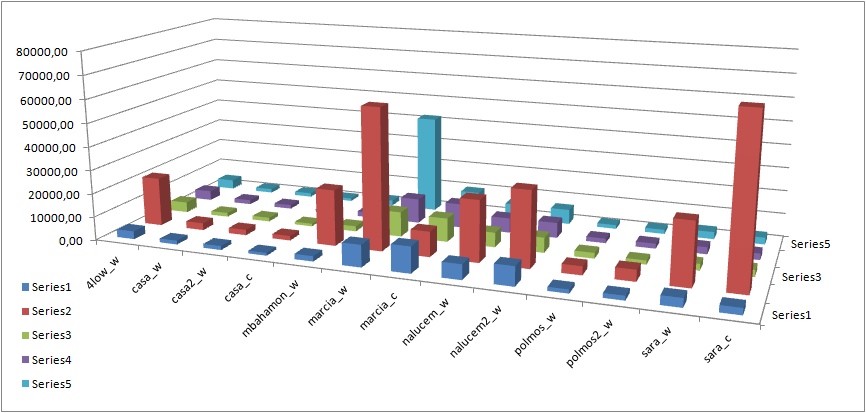
\includegraphics[width=0.9\textwidth]{img/measures_page}
\caption[Page Benchmark: Total Load Means]{ Total Load means (in ms) based on \ref{app:pbmeasures}, Table \ref{table:loadmeans}}
\label{fig:loadmeans}
\end{figure}%

Before realizing that the router was the flaw in the network
\textit{mbahamon\_w}, under conditions of stress, this network was one of the
most affected networks delaying average time 23 seconds. The networks that are
in worst situations are those mentioned \textit{marcia\_w} and
\textit{sara\_c}. Due to the presence of large buffers which store packets of
uncontrolled manner and for longer periods, when the network's load decreases,
this resource  still under utilization. This is reflected in the observations
from from 3 onwards.

\begin{table}[ht]
\begin{center}
\begin{tabular}{|c||c|c|c||}
 \hline
Name 			& min		& max		& ratio  	\\ \hline \hline
4low\_w 		& 3415,1	& 20932,3	& 612,93374 \\ \hline 
casa\_w 		& 1654,8	& 3053,6	& 184,52985 \\ \hline 
casa2\_w		& 1646,6	& 2354,4	& 142,98555	\\ \hline 
casa\_c			& 1165,3	& 1944,1	& 166,83258	\\ \hline 
mbahamon\_w		& 2182,6	& 23868,5	& 1093,58105\\ \hline 
marcia\_w		& 9401,6	& 60119,0	& 639,45499	\\ \hline 
marcia\_c		& 10028,3	& 11140,0	& 111,08563	\\ \hline 
nalucem\_w 		& 6280,8	& 26048,6	& 414,73379	\\ \hline 
nalucem2\_w 	& 6349,4	& 32151,5	& 506,37068	\\ \hline 
polmos\_w 		& 1623,4	& 3701,4	& 228,00296	\\ \hline 
polmos2\_w 		& 1738,5	& 4861,8	& 279,65487	\\ \hline 
sara\_w 		& 2808,6	& 26561,5	& 945,72029	\\ \hline 
sara\_c 		& 2757,6	& 70423,3	& 2553,78953\\ \hline 
\end{tabular}
\caption[Page Benchmark: Minimum, Maximum and variation ratio.]{Minimum, Maximum and variation ratio.}
\label{table:varatio}
\end{center}
\end{table}

In Table \ref{table:varatio}, can be seen the comparison between the minimum
and maximum average load value across over all iterations on the same network
and the ratio between these values. While the ratio can not be compared
directly between two different networks, but can compare how many times the
maximum value was respect to its original value \footnote{a network may have a
low ratio with times that have a low variance and high average time}. Here,
the network \textit{marcia\_c}, and in the Table \ref{table:loadmeans},
accomplish times that were close to 11 seconds for all five iterations. With
this values, the ratio is low (11\%) but the real values are relatively high
for normal conditions (around 11 seconds).

Again, the networks \textit{marcia\_w}, both cases for \textit{sara}, stand
here because the high level of variation around 6 to 20 times the lowest
average time; highlighting \textit{mbahamon\_w} and \textit{sara\_c}. Contrary
to what was expected, in the case of the wired iteration over sara,
\textit{sara\_c}, the maximum variation was significantly higher in this
iterations than for those observed using wireless technology.

\begin{table}[!ht]
\begin{center}
\begin{tabular}{|c||c|c|c|c|c||}
 \hline
 & \multicolumn{5}{|c|}{ Ratio (\%)} \\ \hline
Name 		& 1			& 2			 & 3	        & 4				& 5 			\\ \hline \hline
4low\_w		& 155,55556	& 707,62342	 & 196,64754	& 232,87492		& 3302,32392	\\ \hline
casa\_w		& 108,35366	& 299,26429	 & 116,08775	& 356,49786		& 118,85296 	\\ \hline
casa2\_w	& 113,99878	& 281,65249	 & 127,18041	& 103,10219		& 117,71533 	\\ \hline
casa\_c		& 112,57589	& 304,73684	 & 103,63636	& 103,57766		& 104,58478 	\\ \hline
mbahamon\_w	& 163,95912	& 183,86356	 & 153,77847	& 139,55813		& 319,52128 	\\ \hline
marcia\_w	& 309,24808	& 6298,01469 & 267,57064	& 198,10685		& 205,48759 	\\ \hline
marcia\_c	& 310,36182	& 187,34044	 & 146,11202	& 205,08497		& 138,25129 	\\ \hline
nalucem\_w	& 261,95410	& 254,73473	 & 109,85803	& 106,96041		& 105,23376 	\\ \hline
nalucem2\_w	& 980,66263	& 315,95548	 & 254,12946	& 284,86443		& 110,70346 	\\ \hline
polmos\_w	& 106,36537	& 263,10680	 & 3902,47219	& 8443,23607	& 4150,06459 	\\ \hline
polmos2\_w	& 159,75460	& 1991,19249 & 8206,53009	& 417,45121		& 8226,29199 	\\ \hline
sara\_w		& 402,38095	& 240,75420	 & 394,93299	& 976,89312		& 395,52042 	\\ \hline
sara\_c		& 111,04952	& 281,07638	 & 109,03226	& 107,01366		& 109,54898 	\\ \hline
\end{tabular}
\caption[Page Benchmark: Ratio over own iteration]{Ratio over own iteration.}
\label{table:variationratio}
\end{center}
\end{table}

Also, for some cases adding another source was not decisive to obtain times
quite high. As can be seen in \ref{table:variationratio}, for
\textit{polmos\_w}, which in its latest iteration had a maximum of 127.343 ms
\footnote{The detailed values are available with CD} and a minimum of 1548ms.
Grounds for these outlayers measurements may be due to many factors ranging
from the conection setup to server problems.


\subsection{Smokeping Test}
It is already clearly established the presence of bufferbloat at least three
networks, resulting in a decrease in the performance and usability of the
networks, resulting in catastrophic times of answer for anyone who wants to
have a smooth sesion with any other service that requires capacity of the
network.

Trying to assimilate otherwise these results is that in Figure
\ref{fig:smokenat} can see the contrast of the two opposite poles.

\begin{figure}
\begin{subfigure}{\textwidth}
  \centering
	%\rule{5.5cm}{7.1cm}
    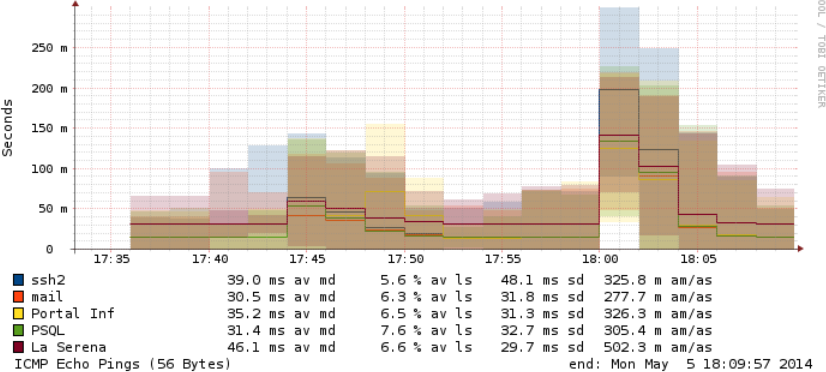
\includegraphics[width=0.8\textwidth]{img/smoke_nat_good}
\caption[Smokeping: Ping test to National servers with good performance]{Good performance Network}
\label{fig:smokenatgood}
\end{subfigure}%
\\
\begin{subfigure}{\textwidth}
\centering
	%\rule{5.5cm}{7.1cm}
    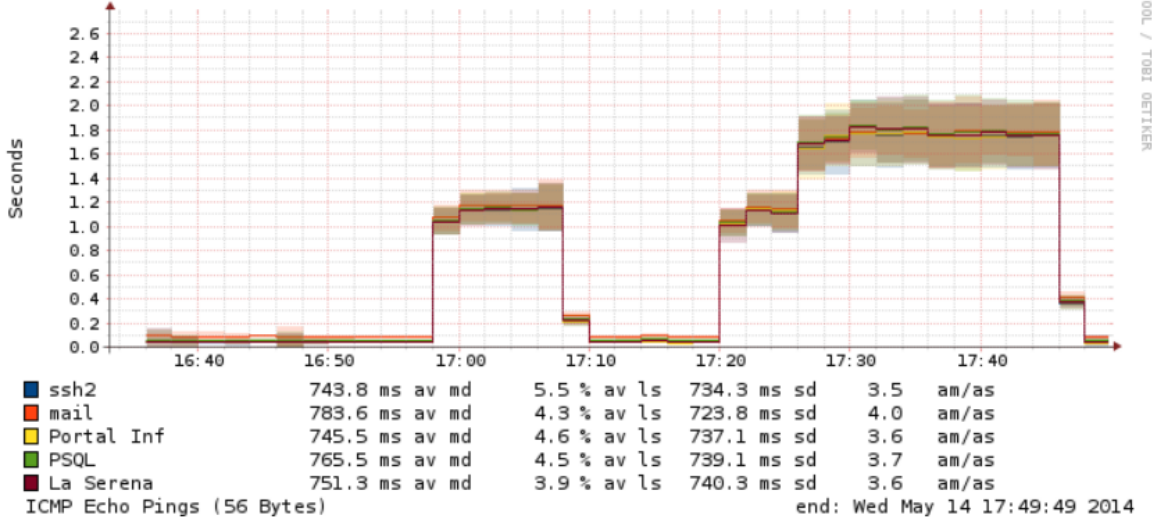
\includegraphics[width=0.8\textwidth]{img/smoke_nat_bad}
\caption[Smokeping: Ping test to National servers with bad performance]{Bad performance Network}
\label{fig:smokenatbad}
\end{subfigure}
\caption[Smokeping: Ping test to National servers]{Ping test to National servers}
\label{fig:smokenat}
\end{figure}

Figure \ref{fig:smokenatgood} shows the behavior of the network
\textit{casa\_w} which has faster response times with  no load around 50ms and
to superor  200ms with maximum use of the network. While can be appreciate
greater amount of \textit{``smoke''} (bar with same color as the line), this
is because by the time range that is driving (very low), tends generates this
small variation.

In contrast, in Figure \ref{fig:smokenatbad}, the amount of smoke is much
lower, but the variation in time is much higher, resulting in lower time to
100ms before loading, then vary drastically reaching over two seconds. While
this case was less packet loss, test took almost the double because of the
tendency to vary dramatically in the second case.


\begin{figure}
\begin{subfigure}{\textwidth}
\centering
	%\rule{5.5cm}{7.1cm}
    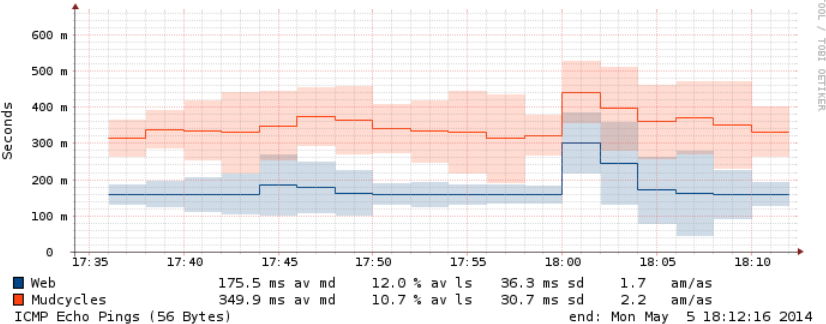
\includegraphics[width=0.8\textwidth]{img/smoke_int_good}
\caption[Smokeping: Ping test to International Servers with good performance]{Good performance network}
\label{fig:smokeintgood}
\end{subfigure}%
\\
\begin{subfigure}{\textwidth}
\centering
	%\rule{5.5cm}{7.1cm}
    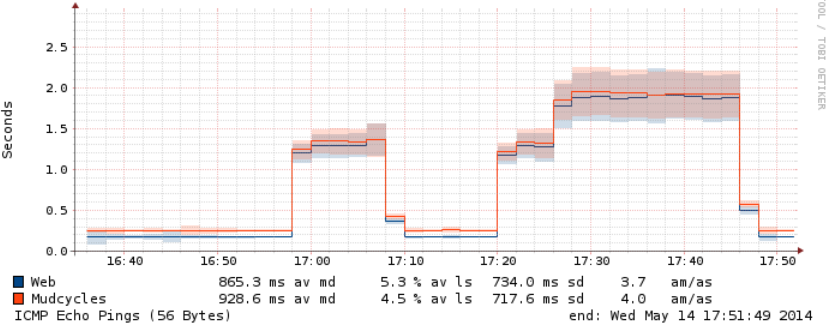
\includegraphics[width=0.8\textwidth]{img/smoke_int_bad}
\caption[Smokeping: Ping test to International servers with bad performance]{Bad performance network}
\label{fig:smokeintbad}
\end{subfigure}
\caption[Smokeping: Ping test to International servers]{Ping test to International servers}
\label{fig:smokeint}
\end{figure}

For international servers, it can be appreciated that the tendency remains
very strong. The times related to Figure \ref{fig:smokeintbad} increases to 8
times its minimum value, ranging from 250ms to about 2 seconds. Again, the
loss in Figure \ref{fig:smokeintgood} is almost double than in Figure
\ref{fig:smokeintbad}, but the latter spent a longer period without load,
which reflect that in average have lower loss.

It is also interesting to note that while both servers are in the U.S., the
requests to the server noticed by the orange line took almost twice the time
against the blue-line-host  (above 300ms). This may be due to the
characteristics of the service provided or the resolution time by the server
because after a little more investigation, it was determined that was hosted
on a VPS with characteristics similars to Iperf's server connection used (same
hosting service).

\begin{figure}
\begin{subfigure}{\textwidth}
\centering
	%\rule{5.5cm}{7.1cm}
    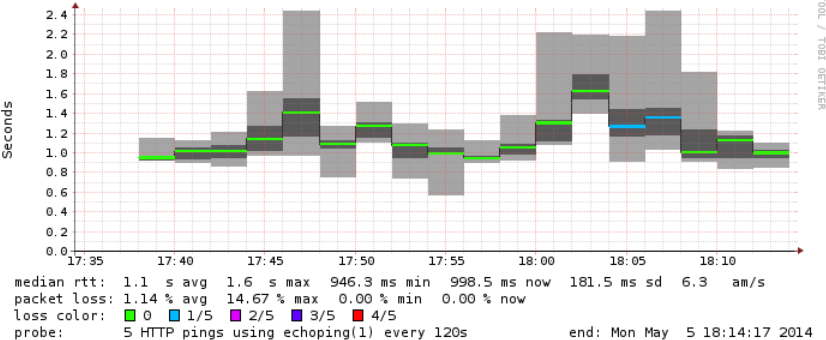
\includegraphics[width=0.8\textwidth]{img/smoke_inf_good}
\caption[Smokeping: Web requests with good performance]{Good performance network}
\label{fig:smokewebgood}
\end{subfigure}%
\\
\begin{subfigure}{\textwidth}
\centering
	%\rule{5.5cm}{7.1cm}
    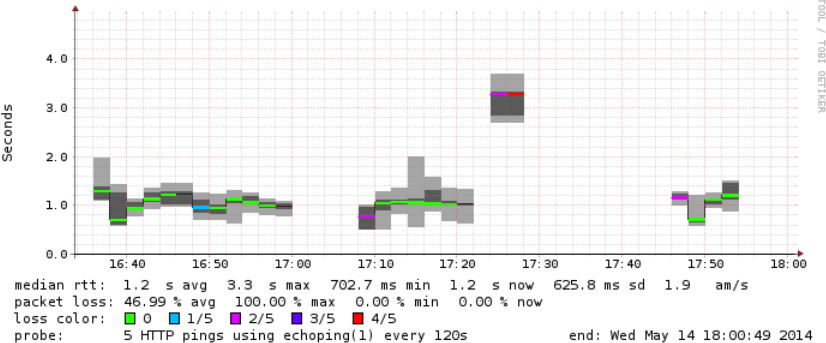
\includegraphics[width=0.8\textwidth]{img/smoke_inf_bad}
\caption[Smokeping: Web requests with bad performance]{Bad performance network}
\label{fig:smokewebbad}
\end{subfigure}
\caption[Smokeping: Web requests to National servers]{Web requests to National servers}
\label{fig:smokeweb}
\end{figure}

To conclude, Figure \ref{fig:smokeweb}  reveal the results of the HTTP
requests. In the case of Figure \ref{fig:smokewebgood}, load average achieved
was 1.1 seconds  with a loss of approximately 1.14\%. In contrast, in Figure
\ref{fig:smokewebbad}, right after the first overload (close at 17:00 hrs) of
the network, communication is affected, only been able to resume the
communication upon completion of the test. In the second iteration, becomes
not only intermittent communication, but also when it generate some traffic,
it takes about 3 seconds and has a loss of about 70\%. This not only affirms
our theory about the behavior and relationship to loss over time that lasted
the test, but also shows how terrible it would be for anyone trying to load
any website.


\subsection{Summarising Results}
The results are synthesized in order to analyze them comprehensively. 
The first test gave us the data to define the bandwidth of each
network with which subsequently went to work. Overall the upload link (uplink)
behaved as expected, performing in some cases gains of up to 50\% or more than
contracted. Obviously this could be due to generally low values ($\sim1Mbps$)
are therefore at a small variance is expressed as a high variation ratio. For
networks with greater uplink, between 1 and 5 Mbps also showed good
performance. On the other hand, the downlink reveal more variation between the
contracted and obtained. The circumstantial differences between a network with
good behavior to those with certain problems got reflected at this point. A
special case was the network \textit{polmos}. Strangelym after being tested with two
different Operating Systems (but on the same computer) results near
the contracted value were never obtained; not with other devices, where exhibit
values around the 40Mbps. The range values for the ping was not as expected,
but they still accepted values without being detrimental to smooth navigation
with a use that does not cause an excessive stress to the system.

With Netalyzr it is possible to obtain a clearer idea of the fundamentals and the
inner workings of networks. Also most revealing information was obtained from
the theoretical perspective, the existence of Bufferbloat obtaining
approximate times of the duration of the buffers present in these networks.
This results was the most important for the continuity of the study, mainly
because it proceeded to rule out or find problems associated with other
factors, for example a defective router (as in the case of \textit{mbahamon})
or environmental interference.

Iperf revealed the behavior of the networks trying to use their full
capacity. Also checked the behavior of the protocols and the different phases
that they have (slow start and congestion avoidance periods). While this was
not within the objectives of the study, witness the behavior helped to verify
that the operating level protocols, were working as expected. Along with this,
it helped to ensure that the presence of buffers is lethal when trying to make
a fluid exchange data with a high level of network utilization.

The simulation of the experience gained by a user when trying to load a
website under periods of low and high loads also can enable to understand
better the effects of Bufferbloat. While the trend was already well defined by
the above tests, individual results included in the study were obtained, but
defined as outliers, such as occurred in the network \textit{polmos\_w} where
a maximal value was obtained in the last iteration, which were expected  to be
more alike to the first iteration.

If it is believed that due to Bufferbloat the times were increased, thanks to
smokeping got demonstrated that not only increase considerably, but almost
impossible to web surf or almost very difficult to think in online games with
good performance. The resulting loss and increased latency are considerable
reaching about 12 times the initial value, and growing to 100\% loss
communication.

%end section Test
\newpage
%section Test
\section{Conclusions and Further Work}
By analyzing all of the work done for this thesis, it is possible to conclude
that the objective of it was achieved considering the same frame of reference
as the criteria defined at the beginning of it being the \emph{objective of
checking the effects of Bufferbloat phenomenon, test the impact that it has in
on different networks and to propose solutions}. To accomplish
this, it first required to address the following general objectives:

\begin{itemize}
	\item To explain the \emph{Bufferbloat} phenomenon, and explain the impact that it could have over latency and throughput in Internet.
	\item To detect the presence by empirical measure of the latency and throughput in a TCP/IP Network.
	\item To propose possible solutions in the implementation of a network where the existence of excessively large and frequently buffers are detected.
\end{itemize}

Thanks to the various tests it was possible to demonstrate the presence and
feel the effects of \emph{Bufferbloat} in some networks. While the common
factor in them at first sight is their low bandwidth, you can not directly
assign this as a cause, as also contrary cases that had a bad performance
determined by physical effects such as routers were in poor condition or
environmental interference.

As proven in this thesis and corroborated in \cite{MathisMacroCAA}, in
general, a low latency network is wanted in order to exchange  messages between a server and a client. Since low latency make us feel
a faster web surfing and enables better performance in online games and VoIP
technology.

It is clear that the farther away a clients is from the server, the latency
will be higher, but what if we put more and more load to the network, how much
the latency can go up to? Having 12 times the latency when the network
overload is not normal and as mentioned by \emph{Jim Gettys} several times,
the culprit is Bufferbloat.

The effects on latency and navigation are catastrophic growing to full
charging time in minutes or even generate timeout sites.  If we take
today's world where it is more and more common to see applications that make use of
high bandwidth, makes it almost impossible navigating multiple users with these
characteristics. Then, two users on the same network using such applications
should take turns to ensure a smooth operation.

Also from \cite{main:ref:1} and \cite{Vu-Brugier}, we can see that the rule-of-thumb of sizing routers $B = (\overline{RTT}xC)$ doesn't longer apply. With
routes which have sizes much larger buffers than required, all it does is slow
down and hinder the passage of trading floors. The larger the buffer size, the
longer it takes for a packet to go through it, not adding any value in the
packet transfer and only adding additional latency.

In the past days networks had much lower performance than they are today,
so as \emph{Bufferbloat} alike phenomena were more difficult to detect
because their effects were not as visible. Today with the advance of
technology and the use of tools that feed us with information almost
instantaneously, any change or modification at any point within the
communication channel is evident, and why not say is magnified even to make
some systems collapse.

The complexity of deploying new algorithms into production environments is
such that no matter how many tests are performed over new algorithms, the
conditions under development environments will hardly match. Also doing testing
in production environments is too hard and too complex\cite{Vu-Brugier},
and if tests are not well designed can affect users in a hard way.

Thanks to Codel, and Bufferbloat community is possible to propose an effective
solution to the phenomenon of Bufferbloat. Although while this phenomenon has been studied for a couple of years, the solutions are not yet fully proven,
but these solutions are designed
for modern systems (e.g.. Codel requires BQL recommended for Linux kernel 3.5
onwards), so there will always be some systems vulnerable to its effects. Apply
QoS and bandwidth limiting for some applications are the
most common and easy to implement recommendations for any user, regardless of
the operating system on which they are working.

It is also important to keep a regular check of all the components in our
networks, not only to our computer. Effects of routers in evil, or using
technologies like wireless with the boom of recent years in homes fact that
interference between emitters is much more common than years ago, can be
determining factors in achieving this long-awaited win the last game shooter,
or close the business of our lives through a video conference.

Much is still to be done in this field. As example, the analysis in specific of
how the three different flows (Elephant, mice and
ant)\cite{HaElephants, evolvshortlongflows} are affected by big buffers
and prioritize smaller flows can help fix some of the issues like DNS
resolution, but how they react when the whole network is under the effects of
\emph{Bufferbloat}? The effects change if this occurs at a last-mile-router
or at a back-bone?

Thanks to studies as done by Hoiland-Jorgensen\cite{TokeLinux}, is that a
better understanding of how the Linux Kernel reacts to \emph{Bufferbloat}, but
this follows up to all Linux based OS? With the advance of technology, new
devices are getting cheaper and most people can have access to them. Well
known is the case of Open-Wrt\cite{openwrt}, that is a Linux distribution for
embedded devices. Projects like Cero-WRT\cite{cerowrt}, can help to the
community to fight against \emph{Bufferbloat} in every piece that is
involved on the communication. But will this help in all devices? As example,
Arduino Yun is a microcontroller board, with an Atheros processor that
supports a Linux distribution based on OpenWrt named OpenWrt-Yun. The board
has built-in Ethernet and WiFi support. So, will this board behave well under
high consumption of bandwidth too? Also the effects of \emph{Bufferbloat}
under Windows machine are not well known. Beside the recommendations of the
Bufferbloat community\cite{windowstips} not much information can be found
about it. Study the effects under laying the use of
CTCP\cite{Tan06compoundtcp}\cite{4146841} will be a good starting point.


%end section Conclusions
\newpage
%%%%%%%%%%%%%%%%%%%%%%%%%%%
%incluyo referencias
\bibliography{references,rfc}{}
%%%%%%%%%%%%%%%%%%%%%%%%%%%%
\newpage
%%%%%%%%%%%%%%%%%%%%%%%%%%%%%%%%
\begin{appendix}
\section{Speed Test Details results}\label{app:bwmeasures}
\begin{table}[ht]
\begin{center}
\begin{tabular}{|c||c|c|c|c|}
\hline
Location  & Medium  & Uplink (Mbps) & Downlink (Mbps) & Ping (ms)\\ \hline\hline
 casa\_w     & Wireless & 4,95           & 15,48         & 18 \\ \hline       % mov 5x15%
 casa2\_w    & Wireless & 5,09           & 13,46         & 20 \\ \hline       % mov 5x15%
 casa2\_c    & Cable    & 5,15           & 15,44         & 19 \\ \hline       % mov 5x15%
 marcia\_w	& Wireless & 0,83	        &  6,3			& 29 \\ \hline
 marcia\_c	& Cable    & 0,83	        &  6,29	        & 29 \\ \hline
 sara\_w	    & Wireless & 0,56	        &  5,45	        & 31 \\ \hline
 sara\_c	    & Cable    & 0,57	        &  8,08	        & 30 \\ \hline
 polmos\_w   & Wireless & 2,32           & 19,61         & 26 \\ \hline       % vtr 2x40%
 polmos2\_w  & Wireless & 2,34           & 18,72         & 22 \\ \hline       % vtr 2x40%
 nalucem\_w  & Wireless & 0,57           & 3,97          & 35 \\ \hline       % mov 0,5x4%
 nalucem2\_w & Wireless & 0,56           & 4,06          & 36 \\ \hline       % mov 0,5x4%
 mbahamon\_w & Wireless & 0,6            & 10,21         & 24 \\ \hline       % vtr 0,5x10%
 4low\_w     & Wireless & 0,6            & 8,03          & 29 \\ \hline       % vtr 0,5x10%
 hidalgo\_2  & Wireless & 1,19           & 17,96         & 19 \\ \hline       % vtr 1x20%
\end{tabular}
\end{center}
\caption[Speed Test: Speeds and Ping measured]{Speeds and Pings measured. }
\label{table:speeds}
\end{table}

\begin{table}[ht]
\begin{center}
\begin{tabular}{|c|c||c|c||c|c||}
\hline
&&\multicolumn{2}{|c||}{Measured (Mbps)} & \multicolumn{2}{|c||}{Contracted (Mbps)} \\ \hline	
Location	& Provider	& Uplink 	  	 & Downlink  &	Uplink	& Downlink \\ \hline \hline 
casa\_w		& Movistar	& 4,95			 & 15,48	 & 5		& 15 \\ \hline 
casa2\_w	& Movistar	& 5,09			 & 13,46	 & 5		& 15 \\ \hline 
casa\_c	 	& Movistar	& 5,15			 & 15,44	 & 5		& 15 \\ \hline 
marcia\_w	& VTR		& 0,83			 & 6,3 	 	 & 0,5		& 10 \\ \hline 
marcia\_c	& VTR		& 0,83			 & 6,29	 	 & 0,5		& 10 \\ \hline 
sara\_w		& Movistar	& 0,56			 & 5,45		 & 0,5		& 10 \\ \hline 
sara\_c		& Movistar	& 0,57			 & 8,08		 & 0,5		& 10 \\ \hline 
polmos\_w	& VTR		& 2,32			 & 19,61	 & 2		& 40 \\ \hline 
polmos2\_w	& VTR		& 2,34			 & 18,72	 & 2		& 40 \\ \hline 
nalucem\_w	& Movistar	& 0,57			 & 3,97	 	 & 0,5		& 4 \\ \hline
nalucem2\_w	& Movistar	& 0,56			 & 4,06		 & 0,5		& 4 \\ \hline
mbahamon\_w	& VTR		& 0,6 			 & 10,21	 & 0,5		& 10 \\ \hline
4low\_w		& VTR		& 0,6			 & 8,03		 & 0,5		& 10 \\ \hline
hidalgo\_w	& VTR		& 1,19			 & 17,96	 & 1		& 20 \\ \hline
\end{tabular}
\end{center}
\caption[Speed Test: Measured and Contracted Speed ]{Measured and Contracted Speed.}
\label{table:comparative}
\end{table}

\newpage
\section{Page Benchmark results}\label{app:pbmeasures}

\begin{table}[ht]
\begin{center}
\begin{tabular}{|c||c|c|c|c|c||}
 \hline
& \multicolumn{5}{|c|}{ Total Load Means (ms)} \\ \hline
Name         & 1		& 2			& 3			& 4			& 5 		\\ \hline \hline	
4low\_w		 & 3415,10	& 20932,30	& 4490,50	& 4170,10	& 4087,10 	\\ \hline	
casa\_w		 & 1654,80	& 3053,60	& 1718,00	& 1877,40	& 1666,80 	\\ \hline
casa2\_w		 & 1682,90	& 2354,40	& 1682,30	& 1667,50	& 1646,60 	\\ \hline	
casa\_c		 & 1191,00	& 1944,10	& 1167,10	& 1165,30	& 1180,90 	\\ \hline	
mbahamon\_w	 & 2248,40	& 23868,50	& 2248,00	& 2182,60	& 2223,80 	\\ \hline	
marcia\_w	 & 9401,60	& 60119,00	& 10692,40	& 10646,70	& 42022,80 	\\ \hline	
marcia\_c	 & 11140,00	& 10764,30	& 10158,80	& 10386,30	& 10028,30 	\\ \hline	
nalucem\_w	 & 6421,40	& 26048,60	& 6280,80	& 6335,80	& 6306,40 	\\ \hline	
nalucem2\_w	 & 8199,00	& 32151,50	& 6479,10	& 6537,10	& 6349,40 	\\ \hline	
polmos\_w	 & 1623,40	& 3701,40	& 2420,60	& 1947,00	& 1659,30 	\\ \hline	
polmos2\_w	 & 1912,40	& 4861,80	& 1738,50	& 2136,10	& 1827,50 	\\ \hline	
sara\_w		 & 3781,30	& 26561,50	& 2808,60	& 3005,30	& 3101,00 	\\ \hline	
sara\_c		 & 2806,50	& 70423,30	& 2865,90	& 2757,60	& 2964,50 	\\ \hline	
\end{tabular}
\caption[Page Benchmark: Total Load Means.]{Total Load Means.}
\label{table:loadmeans}
\end{center}
\end{table}
\end{appendix}

\end{document}
